% Carleton University SCE 4th Year Project thesis style
% University of Ottawa MSc thesis style -- modifications to the report style
% modification of suthesis style of Stanford University
% Example of use:
    \documentclass[12pt]{report}
    \usepackage{amsmath,amssymb,amsthm}
    \usepackage{SCE4YPTemplate}
    \usepackage{graphicx}
    \usepackage{url}
    \usepackage{wrapfig}
    \usepackage{titlesec}
    \usepackage{tabularx}
    \usepackage{booktabs}
    \usepackage{threeparttable}
    \usepackage{float}
    \usepackage{pdfpages}
    \usepackage{enumitem}
\usepackage{subcaption}
    \usepackage{pythonhighlight}

    
    \graphicspath{ {./images/} }
    \newcommand{\sectionAuthor}[1]{{\small\vspace{-1em}\textit{#1}}\bigskip\par}
    % Testing %
    \newcommand\tabularhead[1]{
    \begin{table}[H]
      \caption{Use Case #1}
      \begin{tabular}{|p{0.25\linewidth}|p{0.7\linewidth}|}
        \hline
        \textbf{Use Case Name} & \textbf{#1} \\
        \hline}
    
      \newcommand\addrow[2]{#1 &#2\\ \hline}
    
      \newcommand\addmulrow[2]{ \begin{minipage}[t][][t]{4cm}\raggedright#1\end{minipage} 
         &\begin{minipage}[t][][t]{10cm}
          \begin{enumerate} #2   \end{enumerate}
          \end{minipage} \vspace{0.1cm} \\ \hline}
          
      \newenvironment{usecase}{\tabularhead}
    {\end{tabular}\end{table}}
    
    

    \begin{document}
    
    \title{Carleton University
    \\ Mail Delivery Robot}
    \author{Stephen Wicklund, Emily Clarke \\{\small Supervised by: Dr. Babak Esfandiari, Patrick Gavigan}}
	    % Remember to use your titles
	    % Use \copyrightyear{1885} to force a particular year
	    % for the copyright statement.
     \copyrightfalse % do not produce a separate copyright page
		    % otherwise use \copyrighttrue
%    \figurespagefalse % do not produce a separate figures page
%    \tablespagefalse  % do not produce a separate tables page

% Here you insert the stuff that comes before the preface
% Each preface section is contained in a \prefacesection and starts on a
% new page.  These are numbered using Roman numerals.
% If there are no such pages, do not remove the \beforepreface command
% since it creates the title page.
    \beforepreface

%=================================================================================

%=================================================================================

    \prefaceTOC   % to print the Table of Contents
    \prefaceLOF   % to print the List of Figures
    \prefaceLOT   % to print the List of Tables



\endpreface
	
%%%%%%%%%%%%%%%%%%%%%%%%%%%%%%%%%%%%%%%%%%%%%%%%%%%%%%%%%%%%%%%%%%%%%%%%%%%%%%%%%%
%
%   Now you proceed in report style with chapters, sections, etc.

\chapter{Introduction}
Despite living in a digital world, physical mail delivery continues to be a logistical challenge. The thought of navigating Carleton's tunnels during periods of high traffic is discouraging and can result in late or missed mail. Physical mail is increasingly vital and time sensitive so automating the mail delivery process is more important now than ever. The Carleton University Mail Delivery Robot aims to augment existing mail services and make physical mail as convenient as email.

\section{Objectives}
\subsection{System Overview}
\sectionAuthor{By Emily Clarke}
Mail delivery robots will deliver mail from station to station throughout the Carleton tunnel system. Users will be able to drop off mail at one station, specify which station to deliver mail to, and monitor delivery progress. User access to the system will be provided via a server and web app. Robots will autonomously navigate between stations aided by Bluetooth beacons to determine their location and update the server on their status when able.
\subsection{Functional Requirements}
\sectionAuthor{By Emily Clarke}

\begin{usecase}{SendMail}
    \addrow{Brief Description}{A Sender sends mail to a Recipient.}
    \addrow{Precondition}{System is running and beacons are functioning}
    \addrow{Primary Actor}{Sender}
    \addrow{Secondary Actor}{Recipient}
    \addrow{Dependencies}{Includes DepositMail, ReceiveMail}
    \addmulrow{Basic Flow}{
        \item INCLUDE USE CASE DepositMail
        \item Robot routes path to destination
        \item DO MEANWHILE IF Robot detects obstacle THEN Robot handles obstacle ENDIF
        \item Robot navigates hallway
        \item IF Robot enters intersection THEN Robot navigates intersection to desired hallway according to path ENDIF
        \item IF Robot can communicate with system THEN Robot updates status ENDIF
        \item UNTIL Robot is in destination hallway
        \item Robot goes to and docks with destination receptacle
        \item Robot updates status with System
        \item INCLUDE USE CASE ReceiveMail
        \item[Post.] Mail successfully delivered to Recipient
    }
\end{usecase}

\begin{usecase}{DepositMail}
    \addrow{Brief Description}{A Sender initiates a mail delivery and deposits mail}
    \addrow{Precondition}{System is running}
    \addrow{Primary Actor}{Sender}
    \addrow{Secondary Actor}{Recipient}
    \addrow{Dependencies}{None}
    \addmulrow{Basic Flow}{
        \item Sender submits current location and delivery location
        \item System VALIDATES THAT nearby robot is available \label{validatesAvailable}
        \item System replies with nearest available robot
        \item Sender places mail in robot receptacle
        \item System notifies recipient of upcoming delivery
        \item [Post.] Mail is in robot and recipient notified
    }
    \addmulrow{Specific Alternative Flow - RFS \ref{validatesAvailable}}{
        \item System replies with no available robots
        \item ABORT
        \item[Post.] Sender cannot send mail
    }
\end{usecase}

\begin{usecase}{RetrieveMail}
    \addrow{Brief Description}{A Recipient picks up mail}
    \addrow{Precondition}{Robot is docked at destination with mail and System is running}
    \addrow{Primary Actor}{Recipient}
    \addrow{Secondary Actor}{Sender}
    \addrow{Dependencies}{None}
    \addmulrow{Basic Flow}{
        \item System notifies Sender and Recipient of completed delivery
        \item Recipient retrieves mail from robot receptacle
        \item[Post.] Mail successfully delivered to Recipient
    }
\end{usecase}

\begin{usecase}{CheckStatus}
    \addrow{Brief Description}{A user checks the status of a delivery}
    \addrow{Precondition}{System is running and delivery in progress}
    \addrow{Primary Actor}{User (Sender or Recipient)}
    \addrow{Secondary Actor}{None}
    \addrow{Dependencies}{None}
    \addmulrow{Basic Flow}{
        \item User submits request to view delivery status
        \item System replies with most up to date status of Robot deliveries matching user
        \item[Post.] User is informed of most up to date delivery status
    }
\end{usecase}

\begin{usecase}{AdminStatus}
    \addrow{Brief Description}{An Admin views system status}
    \addrow{Precondition}{System is running}
    \addrow{Primary Actor}{Admin}
    \addrow{Secondary Actor}{None}
    \addrow{Dependencies}{None}
    \addmulrow{Basic Flow}{
        \item Admin submits request to view full System status
        \item System replies with full System status
        \item[Post.] Admin is aware of full System status
    }
\end{usecase}

\begin{figure}[H]
\caption{Use Case Diagram}
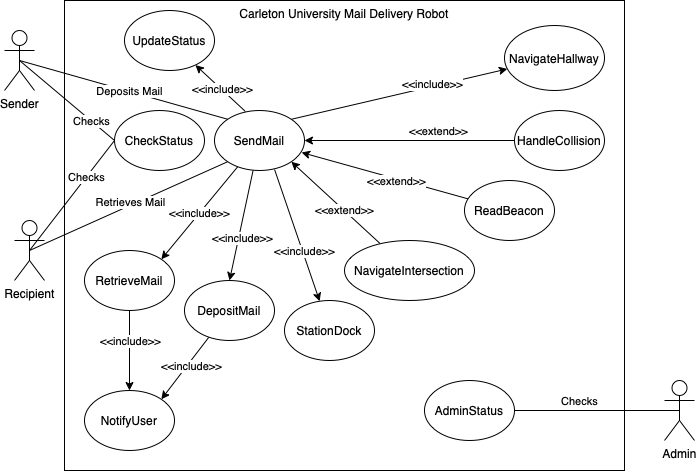
\includegraphics[scale=0.6]{images/UseCaseDiagram.png}
\centering
\end{figure}
\subsubsection{Mail Delivery}
A robot will take mail from Station A in the tunnels to Station B based on user specification.
\subsubsection{Navigation}
A robot can route a path between two locations and then follow walls and navigate intersections until the destination is reached.
\subsubsection{Delivery Status}
Users, both senders and recipients, can check delivery status via a web interface. Delivery status includes whether mail is delivered and last known location of robot.
\subsubsection{Admin Status}
Admins can view full system status via a web interface. Full system status includes last known locations of all robots, reported errors from all robots, and battery levels of beacons. Robots should determine and flag low battery or dysfunctional beacons.
\subsection{Non-Functional Requirements}
\sectionAuthor{By Emily Clarke and Stephen Wicklund}
% \subsubsection{Autonomy}
% Autonomy is a fundamental requirement of the mail delivery system. The system should be able to service a users mail delivery request without any additional user or operator involvement.

% \begin{description}
%     \item[Power Requirements] The robot should operate off batteries which will be able to be recharged autonomously when a robot returns to a station. All onboard device should be powered by these batteries.
%     \item[Course Navigation] A robot should be able to determine a general location based on the signals from nearby active beacons. The robot does not need to be able to determine a specific geographic location, but should be able to make correct navigation decisions based on this information.
%     \item[Tunnel Navigation] The robot will be able to successfully navigate from point A in the tunnels to point B. The robot should always plot the most direct route from point A to point B. Maximum trip time for the test route should be no longer than one hour. Stretch goals will be defined after further testing. 
%     \item[Beacon Maintenance] The amount of beacons used will be kept to a minimum to reduce the initial cost of installation and upkeep. Initially, four beacons per intersection will be used with the goal of reducing it to two and possibly even one.
% \end{description}

\subsubsection{Safety}
The robot should not be a public safety risk to anyone navigating through the tunnels.

\subsubsection{Robustness}
In the event of a collision, inactive beacons or other obstacles, the robot should still make the best possible attempt at delivering the mail. The robot should be able to be pushed to any location in the tunnels and be able to regain course and continue delivery.

\subsubsection{Affordability}
Each robot should be reproducible within a budget of \$500. A minimal amount of beacons should be used to reduce set-up and operational cost.

\subsubsection{Ease of Use}
A first-time user should be able to quickly navigate the web interface and submit a request or monitor a request. The system should not require any training to use.

\subsubsection{Ease of Setup and Maintenance}
An administrative user will be able to construct and deploy a new robot quickly and without frustration. The target for assembly time is one hour with a stretch goal of forty-five minutes. Replacing parts will require minimal time and effort. Repairing any robot should take no longer than thirty minutes for anticipated failures with a stretch goal of fifteen minutes.


\section{Required Skills}
\sectionAuthor{By Stephen Wicklund}
This project requires a range of skills across subjects. This section will discuss what is required and how the group has the capability to undergo the project.

\subsection{Software Engineering}
The project requires the ability to design, build and thoroughly test software systems. The students in the group have developed the skills required through their degree program, Computer Systems Engineering. The following courses: \textit{SYSC1005: Introduction to Software Development}, \textit{SYSC2004: Object-Oriented Software Development}, and \textit{SYSC2006: Foundations of Imperative Programming} allowed the students to develop a range of knowledge of different programming principles. Furthermore, the students completed a medium-sized software and hardware project in \textit{SYSC3010: Computer Systems Development Project}. This project gave the students experience in developing, testing, and documenting a software project.

\subsection{Distributed Systems}
The project requires designing a system which has distributed components that must communicate between each other. This requires expertise in systems design and communication. The students have experience in working with distributed systems when they developed an elevator system in \textit{SYSC 3303: Real-Time Concurrent Systems}. This previous project involved designing a communication model, scheduling and ensuring that all aspects of the system were robust.

\subsection{Embedded Systems}
The robot is an embedded system with power, processing and other constraints which interfaces with a multitude of peripheral devices, this requires a unique set of programming and engineering skills. The students have experience with these types of systems in \textit{SYSC3310: Intro to Real-Time Systems} where they developed knowledge of embedded systems and different I/O implementations.
%%%%%%%%%%%%%%%%%%%%%%%%%%%%%%%%%%%%%%%%%%%%%%%%%%%%%%%%%%%%%%%%%%%%%%%%%%%%%%%%%%
\chapter{The Engineering Project}
\section{Health and Safety}
\sectionAuthor{By Stephen Wicklund}
Throughout the entire course of this project health and safety was prioritized at all levels. The primary concern for health and safety of this project was the ongoing COVID-19 pandemic. Health and Safety issues resulting from the COVID-19 pandemic were addressed by following the Ontario COVID-19 Workplace guide \cite{OntarioCovidPlan} and other local guidelines.
\subsection{Social Distancing}
\sectionAuthor{By Stephen Wicklund}
As outlined in the Ontario COVID-19 Workplace guide \cite{OntarioCovidPlan}, the primary method for eliminating risk of COVID-19 is through elimination, by having everyone work at home. In our group this was done by providing a robot to each group member. The entire setup was replicated and therefore there would be no need to work in person on any aspect of the project.

\section{Engineering Professionalism}
\sectionAuthor{By Emily Clarke}
One important aspect of engineering ethics is not taking credit for other peoples work. Since our project is a continuation of an existing project, we reused a small number of previous scripts. In order to give credit to the original authors, in the analysis chapter there is a section describing what scripts are not our original work (Reuse of ROS Scripts \ref{ROSReuse}).

In addition, engineers have a responsibility to uphold public safety. For this reason we devised methods to ensure the robots are as safe as possible for other tunnel users. These solutions are outlined in the reflections and conclusions chapter (Safety While Moving \ref{safety}).


\section{Project Management}
Due to the size, time-frame and many components of this project, it was vitally important to have proper project management tools in place. The primary tool used was github, both for version control and also issue tracking.
\subsection{Timeline}
\sectionAuthor{By Emily Clarke and Stephen Wicklund}
\label{timeline}
\begin{table}[H]
\centering
\caption{Proposed Timeline for Completion of the Project Milestones}
\centering
\begin{tabular}[t]{lcc}
\toprule
Milestone&Date\\
\midrule
\textbf{Project Proposal}&\textbf{October 22nd}\\
Basic Robot Functionality&November 18th\\
Basic Robot Autonomy&January 14th\\ 
\textbf{Progress Report}&\textbf{January 21st}\\
Intermediate Robot Autonomy&February 28th\\
Full System Demonstration&March 14th\\
\textbf{Final Oral Presentation}&\textbf{March 21st}\\
\textbf{Poster Fair}&\textbf{Cancelled}\\
\textbf{Final Report}&\textbf{April 12th}\\
\bottomrule
\end{tabular}
\begin{tablenotes}
      \small
      \centering
      \item Note: Milestones in bold are hard due dates.
\end{tablenotes}
\end{table}%

\begin{description}
   \item[Basic Robot Functionality] The robot can be controlled by the micro-controller. Wall-following and other scripts can be tested. The robot can read information from the beacons. The web application can be used to send requests.
   
  \item[Basic Robot Autonomy] The robot responds to requests submitted from the web application autonomously. The robot can follow a wall. The robot can determine which beacons are nearby.
  
  \item[Intermediate Robot Autonomy] The robot can receive requests and attempt to navigate to them without assistance, including through intersections. The web application looks functional and is intuitive.
   
   \item[Full System Demonstration] All functional requirements of the system are met.
   
\end{description}
\clearpage
\subsection{Required Components}
\sectionAuthor{By Emily Clarke}
\begin{table}[H]
\centering
    \caption{Required Hardware}
    \begin{tabular}{  l  p{8.5cm} r}
        \toprule
\textbf{Item}      
& \textbf{Description} 
& \textbf{Cost} 
\\\hline
iRobot Create 2
& Robot platform
& \$250
\\\hline
Raspberry Pi 4
& Main controller. 4GB model.
& \$68.75
\\\hline
Raspberry Pi Zero W
& Boot controller
& \$20.94
\\\hline
Buck converter
& Regulate Create 2 robot output voltages to Pi input voltage. Max input of up to 20.5V. Output 5V and at least 3A.
& ~\$5 x2
\\\hline
Inductor
& 2.2mH 1.5A inductor (Ex. Murata 1422514C). Required to use main motor driver on Create 2 robot.
& ~\$6
\\\hline
Wall sensor
& Currently Sharp IR sensors.
& \$15 x2
\\\hline
Bluetooth beacon
& To allow robot to locate intersections. Currently AprilBeacon N04.
& \$10 per
\\\hline
iRobot base station
& To allow robot to charge. One base station is included with each Create 2 robot.
& \$80 per
\\
        \bottomrule
    \end{tabular}
    \begin{tablenotes}
      \small
      \centering
      \item Note: Some cost values are estimates. Tax and shipping is not included.
      \item Note 2: All items are cost per robot except beacons and stations.
\end{tablenotes}
\end{table}

\subsection{Project Risks}
\sectionAuthor{By Stephen Wicklund}
The table below outlines the project risks and mitigation strategies.

\begin{table}[H]
\centering
    \caption{Project Risks and Mitigation Strategies}

    \begin{tabular}{  l  p{8cm}}
        \toprule
\textbf{Project Risk}      
& \textbf{Mitigation strategy} 
\\\hline
Hardware Failure 
& All critical hardware will be replaceable within a reasonable window of time. For items such as beacons or other low cost components, multiple components can be purchased for redundancy. For other components, availability and cost will be considered so that they may be replaced within budget. 
\\\hline
Unable to Access Testing Sites 
& Each group member has access to their own testing equipment. In the event that a testing site cannot be accessed, each member will be able to test the system independently in their own testing area.
\\\hline
The ``Bus Factor"   
& In the event that one group member is unable to continue the project, this should not cause any of their work to be lost. To prevent this all team members will document their work thoroughly and continuously. All work will be stored on the GitHub repository or other cloud-based version controlled solutions. Furthermore, both students will always be participating in all aspects of the project. To facilitate this, pull requests will be made for new additions and code reviews will be conducted before they are merged.
\\\hline
Over-budget/Inflating Project Costs
& Hardware solutions to problems should be simple, easily reproduce-able and cheap. This should allow any needed hardware additions to be reproduced on both robots and any hardware failures to be replaced without going over budget.
\\
        \bottomrule
    \end{tabular}
\end{table}


%=================================================================================

\subsection{Project Planning and Organization}
\sectionAuthor{By Emily Clarke}
The previous team struggled with closely collaborating on all aspects of the project and integrating individual work together. The result of this is that their completed project is disjointed and it is unclear how to run it all at once. In order to avoid these issues, the following project management specific principles should be met:
\begin{itemize}
\itemsep0em 
    \item Every team member generally understands all aspects of the project
    \item To-do tasks are clearly laid out and who is currently working on what is visible
    \item A historical view of progress is available for review
    \item A strong emphasis on agile development principles
    \item No completely independent changes
\end{itemize}
\subsubsection{Issue Tracking}
To ensure all necessary tasks are tracked, every todo item will be created as a GitHub issue. Issues will be assigned to project member(s) so that it is clear who is working on what at which time. In addition, an individual member can quickly filter only their issues. As well, only issues without an assignee can be filtered in order to see if there are any issues that are being ignored or forgotten about. This should decrease the likelihood that important issues are missed and make it much easier to view who is working on what.
\subsubsection{Issue Filtering}
Issues also have the ability to be labelled for quick filtering. One custom label that will be implemented is a “have discussion” label. This will be used during team meetings to quickly pull up a list of what team members want to discuss. This will ensure that issues that need a team discussion won’t be forgotten about and potentially pushed into the future.
\subsubsection{Weekly Project Board}
GitHub issue tracking will be integrated with a weekly GitHub project board. This will show which issues are being worked on for the week in an agile development Kanban view. This is an ideal view for quickly getting an idea of project progress, making it easier and faster to make decisions for what to work on or while reviewing the past week's progress. In addition, we will automate the GitHub project board to match actions in the repository. For example, automatically moving an issue to the “done” column and closing it when the linked pull request is approved and merged. This will reduce project management overhead and free up time to focus on coding. Past boards will remain view-able so project management issues can be identified and solutions implemented on a recurring, agile basis.
\subsubsection{Code Review and Collaboration}
The GitHub repo will be set up to prevent a merge to main without approval from a different team member. This will force code review and increase general understanding of the project for all team members. Importantly, this will prevent only a single team member from having knowledge of a piece of code.




\subsection{Repository Structure}
There is not a need to create multiple repositories for different components of the project since no component is completely independent of one another. Furthermore, by organizing all components into a single repository, we have a “single source of truth”. This will make it easier to more closely collaborate, share and verify code, and refactor when needed. The organization of the project is a single mono-repo with each component being a top-level directory. The top-level directories are as follows:
\begin{description}
    \item[data-analysis] All the data analysis tools, scripts for collecting data about the project.
    \item[mail\_delivery\_robot] The ROS module for the project. This directory contains all components needed to run on the robot.
    \item[webserver] The web application along with the back-end used to send requests and handle communications.
    \item[documentation] Copies of the report and other relevant documentation.
    
\end{description}

\section{Justification of Suitability for Degree Program}
\sectionAuthor{By Stephen Wicklund}
Computer Systems Engineering is a degree program which focuses on "combining hardware and software to design and implement integrated computer systems for applications in such areas as robotics, artificial intelligence, aerospace and avionic systems, multimedia applications and cloud computing". Computer Systems Engineering develops skills in software engineering, analog and digital electronics, computer systems and engineering principles.

This project will involve thoroughly designing and building a system with hardware and software components, following proper engineering principle, and documenting and discussing the process.

A key aspect of the project is proper requirements elicitation and specification, software design and validation and verification. To accomplish this tools such as UML and other system modelling methods will be used. These skills are a focus of \textit{SYSC 3020: Introduction to Software Engineering}.

Furthermore, the robot system will be a distributed concurrent system. The software design will require a communication protocol, multiple threads and a scheduling system. These skills are a focus of \textit{SYSC 3303: Real-Time Concurrent Systems}.

Another aspect of the project is sensors, beacons and other I/O devices. The robot will need to interface with these peripherals and utilize interrupts and other I/O implementation strategies. The entire system is wireless and therefore must operate within power, processing and other constraints. These skills are a focus of \textit{SYSC 3310: Introduction to Real Time Systems}.

The Computer Systems Engineering degree program focuses on developing these skills through designing and implementing systems, such as the one in this project. Over the course of this project, the students will be able to apply these skills and integrate different aspect of the degree program into a single project.

\section{Individual Contributions}
\subsection{Project Contributions}
\subsubsection{Stephen Wicklund}
\begin{itemize}[itemsep=1mm, parsep=0pt]
    \item Tested and analyzed IR Sensors.
    \item Setup structure and configuration of ROS carleton\_mail\_delivery package.
    \item Created robotDriver node, captain node,  beaconSensor node and bumperSensor node.
    \item Updated into ROS2 IRDistanceSensor node and actionTranslator node.
    \item Created data analysis tools for the robot driver.
    \item Designed robot driver state machine and junction traversal behaviour.
    \item Designed collision response behaviour.
\end{itemize}

\subsubsection{Emily Clarke}
\begin{itemize}[itemsep=1mm, parsep=0pt]
    \item Investigated and prototyped beacon reading methods.
    \item Investigated and designed power system.
    \item Designed and prototyped all web interface components.
    \item Planned junction traversal behaviour.
    \item Designed and implemented path finding algorithm.
    \item Integrated path finding and beacon detection into captain node to allow full system functionality.
    \item Designed and implemented variable tuning system for per-robot calibration.
\end{itemize}
\subsection{Report Contributions}
Written report contributions are given as bylines below each section. Refer to the above Project Contributions section for underlying work contributions.
\chapter{Background}
\section{Project History}
\sectionAuthor{By Stephen Wicklund}
This project was first outlined in 2019 in the paper \textit{Toward Campus Mail Delivery Using BDI}\cite{PatrickPaper} by Chidiebere Onyedinma, Patrick Gavigan and  Babak Esfandiari. The paper explore automated systems utilizing Belief-Intention-Desire system and realized in a real-world environment using iRobot Create robots and ROS. The autonomous mail delivery system was continued in  2020 by another group of students at Carleton University in their project, \textit{Autonomous Mail Delivery Robot in University Tunnels}. This project will be a further continuation towards the goal of a fully autonomous mail delivery system in the Carleton University tunnels.
\section{Robot Operating System}
\sectionAuthor{By Stephen Wicklund}
ROS is a set of libraries and tools for developing robotic applications. ROS is a distributed and modular framework made up of many high quality user contributed ``ROS Packages". ROS uses software nodes and publisher-subscriber model and socket-based communications. The publish-subscribe pattern allows senders, called publishers to categorize messages into classes without knowledge of the receivers, called subscribers. Subscribers subscribe to classes they have interest in and receive only messages of that class. Therefore, developers only need to consider the classes they are subscribing or publishing to, and not all the interactions.
\section{iRobot Create 2}
\sectionAuthor{By Emily Clarke}
The iRobot Create 2 is an educational robotic platform designed to be affordable and extensible. It provides a serial interface to allow for specific control of the robots motors and sensors or alternatively the ability to trigger a variety of existing behaviours. 

One such behaviour is the ability to automatically dock with the included charging station. This allows developers to focus on  their specific application and to not need to consider how to implement common behaviours such as charging.

The iRobot Create 2 has built in sensors that are useful for object avoidance and tamper indication. Bumper sensors indicate when there is an obstacle and wheel drop sensors can indicate a ledge has been reached or the robot has been picked up. These built in sensors greatly reduce the assembly complexity of a project using this platform.
 %=================================================================================
% \chapter{Project Management}
%  Other implementations of automated mail delivery use vacuum tubes or conveyor belts. Unfortunately, both of these solutions are infeasible when retrofitting to existing infrastructure. This is where the Carleton University Mail Delivery Robot aims to improve on the existing system of human delivery without any major changes to the existing infrastructure.
%  \clearpage

%=================================================================================
\chapter{Analysis}
In order to better understand the software and hardware tools, a series of experiments and investigations was conducted. These experiments are their findings are outlined in this chapter.
\section{Autonomous Delivery Robot}
\subsection{IR Sensors}
\label{IRSensorTest}
\sectionAuthor{By Stephen Wicklund}
A series of tests was conducted to determine the distance that the IR sensors function at. The goal is to determine a rough minimum and maximum distance and determine the accuracy so that thresholds and a wall-following distance can be chosen.
\subsubsection{Test \#1}
The sensors were placed 30cm away from the wall at a 90\textdegree angle.
\begin{center}
\begin{tabular}{ |c|c| } 
\hline
\multicolumn{2}{|c|}{Distance}\\
\hline
 Mean & 27.25 \\ 
 Standard Deviation & 1.80\\
 Maximum & 30.7\\
 Minimum & 25.4\\
 \hline
\end{tabular}
\quad
\begin{tabular}{ |c|c| } 
\hline
\multicolumn{2}{|c|}{Angle}\\
\hline
 Mean & 78.86 \\ 
 Standard Deviation & 5.25\\
 Maximum & 103.37\\
 Minimum & 52.94\\
 \hline
\end{tabular}
\end{center}

\subsubsection{Test \#2}
The sensors were placed 15cm from the wall at a 90\textdegree angle.
\begin{center}
\begin{tabular}{ |c|c| } 
\hline
\multicolumn{2}{|c|}{Distance}\\
\hline
 Mean & 14.70 \\ 
 Standard Deviation & 0.078\\
 Maximum & 15.17\\
 Minimum & 14.24\\
 \hline
\end{tabular}
\quad
\begin{tabular}{ |c|c| } 
\hline
\multicolumn{2}{|c|}{Angle}\\
\hline
 Mean & 113.16 \\ 
 Standard Deviation & 1.58\\
 Maximum & 122\\
 Minimum & 105.96\\
 \hline
\end{tabular}
\end{center}

\subsubsection{Test \#3}
The sensors were placed 23cm away from the wall at a 45\textdegree angle.
\begin{center}
\begin{tabular}{ |c|c| } 
\hline
\multicolumn{2}{|c|}{Distance}\\
\hline
 Mean & 18.84 \\ 
 Standard Deviation & 0.084\\
 Maximum & 19.50\\
 Minimum & 18.43\\
 \hline
\end{tabular}
\quad
\begin{tabular}{ |c|c| } 
\hline
\multicolumn{2}{|c|}{Angle}\\
\hline
 Mean & 113.16 \\ 
 Standard Deviation & 1.58\\
 Maximum & 122\\
 Minimum & 105.96\\
 \hline
\end{tabular}
\end{center}

\subsubsection{Test \#4}
The sensors were placed 76cm away from the wall at a 90\textdegree angle.
\begin{center}
\begin{tabular}{ |c|c| } 
\hline
\multicolumn{2}{|c|}{Distance}\\
\hline
 Mean & 26.89 \\ 
 Standard Deviation & 0.161\\
 Maximum & 27.69\\
 Minimum & 26.33\\
 \hline
\end{tabular}
\quad
\begin{tabular}{ |c|c| } 
\hline
\multicolumn{2}{|c|}{Angle}\\
\hline
 Mean & 128.51\\ 
 Standard Deviation & 0.91\\
 Maximum & 131.6\\
 Minimum & 123.49\\
 \hline
\end{tabular}
\end{center}
\subsubsection{Conclusion}
It appears the sensors are use-able within approximately 10-50cm of the wall. Beyond that, the distance is not accurate. For best results, we may want the robot to maintain around 15cm from the wall at all times. When the robot was over 50cm from the wall, it read ~25-30cm. If we maintain 15cm from the wall and have the robot search for the wall when it exceeds this distance, it may work fine.

\section{Instrumented Environment}
\subsection{Beacon Experiment 1}
\sectionAuthor{By Emily Clarke}
Three April N04 beacons were placed in a straight line, approximately five meters apart in separate rooms. Proximity and signal noise (rssi) were measured using the manufacturers app on an iPhone 13 Pro. The beacons tx power was set to the maximum (4dB).
\begin{description}
    \item[Location Accuracy] The proximity values for the three beacons consistently were in the correct order based on phone distance to each beacon. When considering an individual beacon, the proximity values frequently changed with up to a 50\% margin of error. This suggests the relative values from multiple beacons are reliable; however, the individual proximity values are not. That being said, an individual value can be used to determine if approaching or departing from a beacon. To get the most accurate proximity value, several samples, for example five, will be taken and then averaged with the outliers discarded. The exact number of samples will be decided on based on testing during implementation. In addition, there was an observed issue where the value will rapidly ramp up or down without any phone movement. To combat this, a maximum standard deviation will be used to discard this behaviour. 
    \item[Connection Distance] Proximity values were received from the highest distance tested, approximately fifteen meters without line of sight. In the tunnels with less obstruction, the actual distance is likely to be much higher; theoretically up to 30 meters according to the manufacturers documentation.
    \item[Beacon Battery] Battery values for the beacons are readable through the app. These values are also readable using the SDK. One limitation is the app cannot reliably get additional information, such as battery, when the beacon is further than approximately five meters away. It is unclear if the SDK has this same limitation although five meters should be sufficient regardless. 
\end{description}
\subsection{Beacon Experiment 2}
\label{BeaconExperiment2}
\sectionAuthor{By Emily Clarke}
A Raspberry Pi 4 was placed in a static location in a hallway. An April N04 beacon was placed at intervals of 1.5m in a straight line away from the Raspberry Pi 4 in the range of 1m to 11.5m. RSSI values for the beacon were recorded by the Raspberry Pi 4 every second. This process was repeated identically for a second beacon.
\subsubsection{Setup}
\begin{figure}[H]
    \centering
    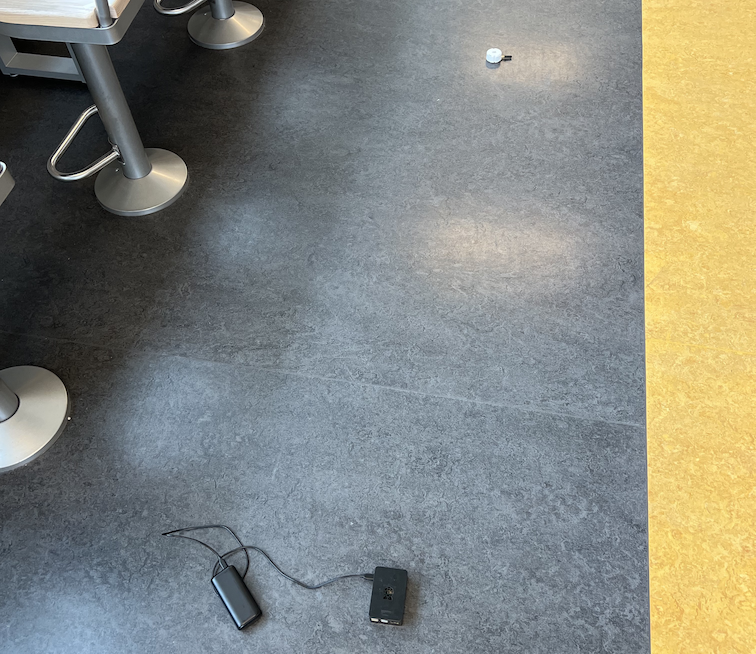
\includegraphics[scale=0.24]{images/rssi-experiment-setup.png}
    \caption{RSSI experiment setup}
    \label{RSSI Experiment Setup}
\end{figure}
\subsubsection{Results}
\begin{figure}[H]
    \centering
    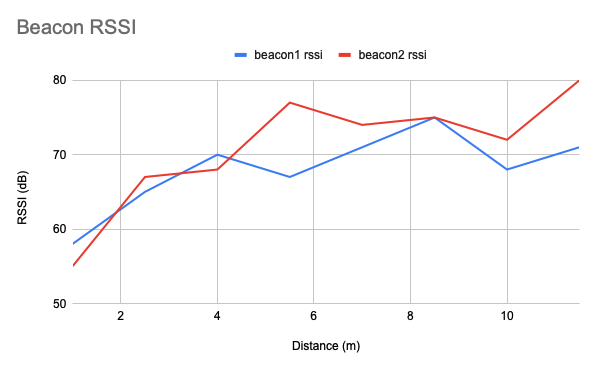
\includegraphics[scale=0.7]{images/rssi-experiment.png}
    \caption{RSSI vs known distances for two beacons}
    \label{RSSI Experiment Plot}
\end{figure}

Initial analysis of the data confirms previous conclusions that a single RSSI value cannot be used to accurately indicate distance; however, there is a clear trend of increasing RSSI over distance as expected. Averaging out experimental results should allow for approximate distance estimates if that is necessary, although this is not planned.

\subsection{Beacon Placement}
\sectionAuthor{By Emily Clarke}
In order to minimize the number of beacons, it is ideal for the robots navigation system to not require connection to a beacon at all times. Since the tunnels have few intersections, the main purpose of the beacons should be to help the robot navigate down the correct hallway at an intersection. Based on the experimental results, relative proximity values for two beacons are reliable. In addition, the robot should be able to determine if it is approaching or departing from a beacon. One possible setup for beacon placement is putting a beacon slightly down each tunnel at an intersection. The robot can then know it is approaching an intersection when the beacon in its current tunnel comes into range. This will let the robot know what intersection it is approaching and from which tunnel. Based on that information, the robot should be able to determine if it needs to go straight or turn after it stops detecting the wall it is following. The relative proximity values for the beacons should allow the robot to determine if it successfully traversed the intersection or if it needs to turn around and try again. It is possible that only two beacons are needed for a standard 4 direction intersection to determine the same information. In addition, a single beacon with passive RFID tags along the walls right before intersections is likely a lower cost alternative that may also perform more reliably.

\section{Robot Operating System}
\sectionAuthor{By Stephen Wicklund}
Robot Operating System (ROS) was selected as a software tool to manage the robot. ROS is a collection of software frameworks. It works off a node based principle where multiple nodes can be run with different tasks. If a single node crashes or is not run, the rest of the system can continue. Nodes communicate with each other using a publish-subscribe pattern.


\subsection{Reuse of ROS Scripts}
\label{ROSReuse}
As a collection of different packages and libraries, before designing the system tools and scripts that could be reused were first selected. The following ROS scripts have been used in the previous project and will be reused.
\begin{table}[H]
\centering
\caption{Reusable ROS Scripts}
\centering
\begin{tabular} { | p{4cm} | p{8cm} | }
\hline
Script Name & Description \\
\hline
IRDistanceCalc.py & Reads the IR Sensors and determines a distance from the wall. This will be used to enable the robot to follow a wall. \\
\hline
BumperSensor.py & Reads the status of the robot's bumper. This will be used to determine when the robot has collided with an object. \\
\hline
driverBluetooth.py & Reads Bluetooth information from the environment. This will be used to read data from the beacons and allow the robot to determine a course. \\
\hline
actionTranslator.py & Converts roomba movement messages into iRobot Create compatible messages. \\
\hline
\end{tabular}
\end{table}%

\subsection{Create Autonomy}
Create\_autonomy is a ROS driver for the iRobot Create1 and iRobot Create2. It will allows commands to be sent from ROS nodes to the create platform to execute actions. 

Using the basic implementation of the Create Autonomy module, the following required features have been confirmed to work on the Create 2 robot:
\begin{itemize}
  \item Automatic dock
  \item Mode control (Forcing manual mode)
  \item Manual movement at chosen speed in supported directions
  \item Safety sensor readings
\end{itemize}
\chapter{Design}
The mail delivery system can be broken up into three subsystems:
\begin{description}
    \item[Autonomous Delivery Robot] The autonomous delivery robot will be built off the iRobot Create platform and uses a Raspberry Pi 4 and sensors to navigate. The purpose of the autonomous delivery robot is to autonomously navigate through the tunnels to fulfill delivery requests. As there is no central controller the robot also will perform all path-finding computations and scheduling in a decentralized manner.
    \item[Web Interface] The web interface will be composed of a web application and a database. The web application is the user interface and platform for submitting delivery requests, monitoring the robots and checking the status of the system. Closely connected to the web application will be a database, which stores requests and relays information between the robot and web application.
    \item[Instrumented Environment] In order for the robot to navigate in the tunnels without access to GPS, the environment needs to be instrumented to allow the robot to determine its position. This will be done with a series of active Bluetooth beacons positioned at junctions in the tunnels, the robot can determine which beacons are nearby and make navigation decisions based off this data.
\end{description}
%=================================================================================
\clearpage
\section{Autonomous Delivery Robot}
  \sectionAuthor{By Stephen Wicklund}
  
The autonomous delivery robot delivers mail, navigates autonomously, schedules requests and performs most system operations. It only requires communication with the other subsystems when it needs additional information about its environment, such as information from beacons or when the robot is idle and requires additional requests to be fulfilled.

\subsection{Robot Operating System}
\sectionAuthor{By Stephen Wicklund}

Robot Operating System (ROS) will function as the software platform that will be the brains of our robot. Through the ROS subscriber-publisher model, the gathering of information and the use of this information can be decoupled. In our project for example, scripts which read sensor information and the scripts which control navigation of the robot can then also be decoupled. This will allow us to easily re-use scripts from the previous work done on the project and integrate seamlessly.

The following information needs to be gathered by the robot:
\begin{itemize}
\itemsep0em 
\item Requests from the server
\item IR sensor data for wall following
\item Beacon data for determining course
\item Bumper Data for determining collision
\end{itemize}

Using the information gathered, the robot then needs to make navigational decisions. The following navigational decisions need to be made by the robot:
\begin{itemize}
\itemsep0em 
\item Plotting a route from Point A to Point B
\item Following a wall to maintain course
\item Making turns at intersections
\item Navigating around obstacles after collisions
\item Docking for charging
\end{itemize}

Each of the items above can be broken into separate ROS scripts, some of which we can reuse from previous work done on this project.

\subsubsection{Additional ROS Scripts}
The following ROS scripts will be created for this project.
\begin{table}[H]
\centering
\caption{ROS Scripts}
\centering
\begin{tabular} { | p{4cm} | p{8cm} | }
\hline
Script Name & Description \\
\hline
ReceiveRequest.py & Receives and stores requests received from the web server.\\
\hline
PlotNavigation.py & Determines a route from point A to point B of the current request. This involves determining all the intersections to turn at. This can be recalculated if the robot gets lost.\\
\hline
RobotDriver.py & Uses the plotted navigation map, beacon information and IR sensors to follow a wall until the desired intersection and then makes a turn. \\
\hline
Captain.py & Uses the navigation data and the navigation map to keep track of the robot with relation to the map. Determines if the robot is off course and the map needs to be recalculated or if beacons are missing or non-functional. \\
\hline
UpdateStatus.py & Sends an update to the web server with the current location of the robot.\\
\hline
DockRobot.py & Navigates to a docking station and charges the robot.\\
\hline
\end{tabular}
\end{table}%

\subsubsection{ROS System Overview}
\sectionAuthor{By Stephen Wicklund}
The ROS scripts are each independent nodes which publish and subscribe to different topics. Should a single node be non-functional, crash or its related sensor be offline, the rest of the nodes can keep operating. Each node subscribes to the topic it requires to function and publishes its output to the topic for other nodes to use.

The complete ROS architecture will be a combination of new nodes created for this project and scripts that are reused from previous projects, as described in section \ref{ROSReuse}.

The ROS Node Map below outlines how the nodes are related in the system. Nodes are shown as rectangles and topics as circles. Robot\_driver is the main navigational node. It reads topics preceptions, bumpEvent, navigationMap and determines what actions the robot should perform, these would be to turn left, stop, reverse, etc. These actions are read by action\_translator and published to cmd\_vel. The create\_autonomy library reads cmd\_vel and executes commands on the robot.

\begin{figure}[H]
\caption{ROS Node Map}
\centering
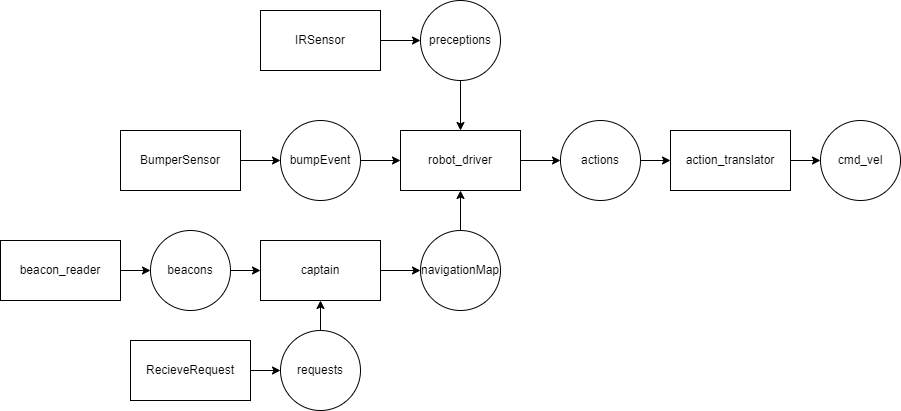
\includegraphics[scale=0.5]{images/ROS Node Diagram Design.png}
\centering
\end{figure}
Note: Nodes are represented with rectangles and topics with circles.

\subsection{Navigation Overview}
\sectionAuthor{By Stephen Wicklund}
A key aspect of the mail-delivery system is the robot's ability to navigate from point A to point B. This is done in two primary stages; Tunnel Navigation and Wall Following Navigation.

Tunnel Navigation is the robot's ability to plot a course from point A to point B. This involves determining which junctions to turn at, which walls to follow and creating an efficient path.

Wall Following Navigation is the robot's ability to travel along a wall from one junction to another, perform turning maneuvers at these junctions and determine its current location by analyzing beacons.

Both of these are explained in the following two subsections.
\subsection{Tunnel Navigation}
\sectionAuthor{By Stephen Wicklund}

The tunnel navigation uses a series of junction objects which when combined create a map of the tunnels. A junction is a representation of a physical location in the tunnels and has beacons attached at each of the entrances to the junction. Below is the physical and database representation of a junction.

The junction database object contains a junction ID and four sections; north, south, east and west. These sections are not real world physical indicators of the positions of the beacons, but are used to represent how the beacons and junction exits are related to each other. For example, if arriving from a southern junction entrance, a left turn is required to exit the junction to the western destination.

Each section contains a beacon ID, which is the MAC address of the beacon and can be read from the robot, the destination junction, which is the next junction the robot will arrive at in that direction and an approximate distance to that junction.

\begin{figure}[H]
\caption{Junction Diagram}
\centering
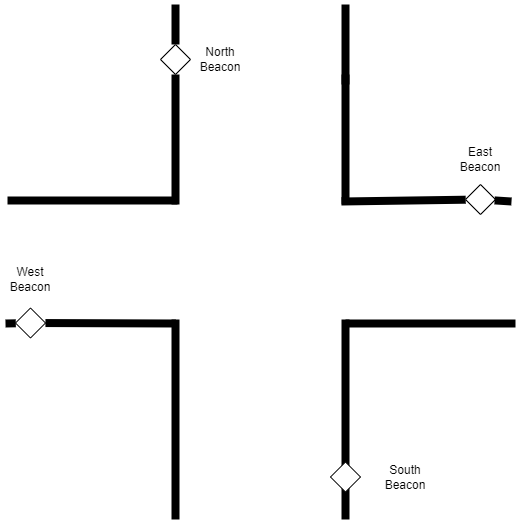
\includegraphics[scale=0.6]{images/Junction Diagram.png}
\centering
\end{figure}

\begin{table}[H]
\centering
\caption{Database Junction Table Row}
\centering
\begin{tabular} { | p{1.5cm} | p{3cm} | p{3cm} | p{3cm} | p{3cm} | }
\hline
Junction ID & North & East & South & West\\
& \{Beacon ID, & \{Beacon ID, & \{Beacon ID, & \{Beacon ID, \\
&DestJunction,&DestJunction,&DestJunction,&DestJunction,\\
&Distance\}&Distance\}&Distance\}&Distance\}\\
\hline

\end{tabular}
\end{table}%

\subsubsection{Path Finding Algorithm}
Now that the junctions are established as a data structure, we can use a basic path finding algorithm to find the shortest path between any two junctions.

\subsection{Wall Following Navigation}
\sectionAuthor{By Stephen Wicklund}

Once the robot has determined the path from its current location, it must then navigate through the tunnels, from junction to junction to its destination. This is done by following walls at an appropriate distance and waiting until it can detect a beacon signalling the approach of a tunnel junction. When the robot approaches tunnel junctions it performs maneuvers to ensure that it leaves the junction in the appropriate direction.

\subsubsection{Traversing Junctions}
An important aspect of tunnel navigation is traversing junctions. The robot can determine when it is approaching a tunnel junction by reading information from nearby beacons. When the robot passes a beacon, it transitions to a junction traversing state and modifies its behavior to both safely traverse the junction and make the correct navigational decisions. There are several challenges when traversing junctions. The robot must maintain the proper course through the changing environment and since the robot can only determine information about its environment through the beacons and the IR sensors mounted on the right of the robot, it will have difficult navigating if it passes a location with no wall to its right. Tunnel junctions may also be areas of high foot traffic, the robot has a higher likelihood of collision if it gets lost in the junction. To mitigate these risks and limit the amount of time the robot is in a high risk position, three Junction Traversal states have been designed.


\begin{figure}[H]
\caption{Junction Pass Through}
\centering
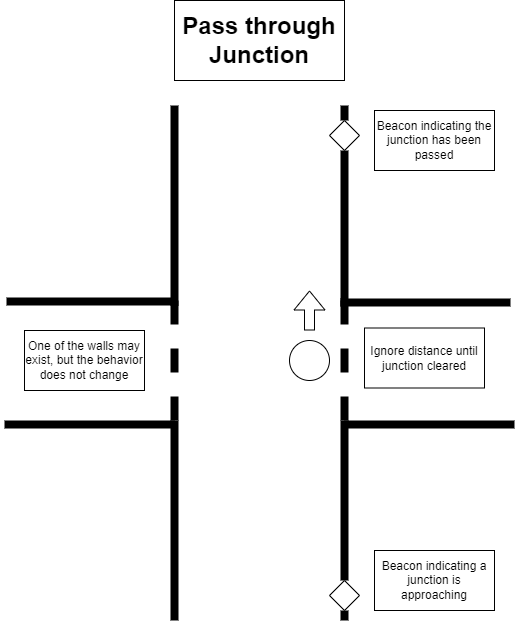
\includegraphics[scale=0.6]{images/Junction Diagrams Pass Through.png}
\centering
\end{figure}

The Junction Pass Through state is the simplest traversal of a tunnel junction. The state is entered when the robot passes the junction entry beacon and determines that it should pass straight through the junction. The robot then navigates straight, stays its course and ignores the distance from the IR sensors in order to navigate past tunnel openings it should not enter. Once the robot approaches the exit beacon it has successfully navigated the tunnel junction and returns to the wall-following state.

\begin{figure}[H]
\caption{Junction Right Turn}
\centering
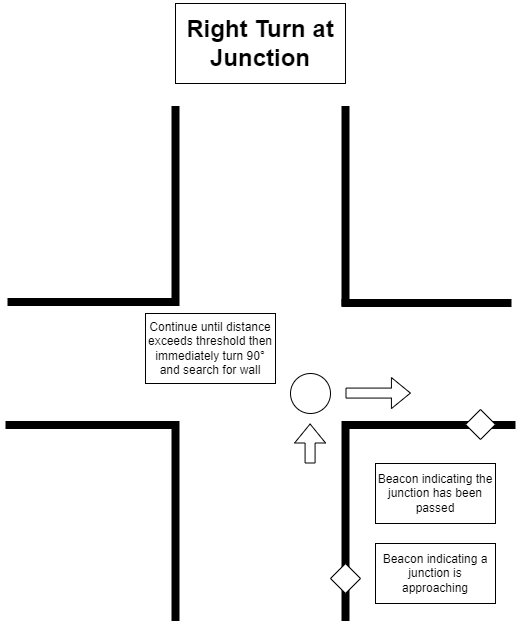
\includegraphics[scale=0.6]{images/Junction Diagrams Right Turn.png}
\centering
\end{figure}

The Junction Right Turn state is entered when the robot passes a junction entry beacon and determines that it should make a right turn at the junction. The robot then continues following the wall until the distance reading from the IR sensor exceeds its threshold, at this point it can make a 90° turn, move forward and quickly resume wall following. Once the robot passes the exit beacon, it resumes its normal wall following state.

\begin{figure}[H]
\caption{Junction Left Turn}
\centering
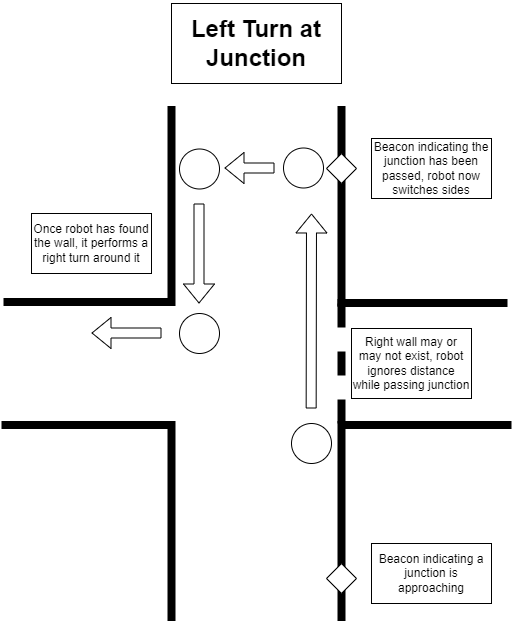
\includegraphics[scale=0.55]{images/Junction Diagrams Left Turn.png}
\centering
\end{figure}

The Junction Left Turn state is entered when the robot passes a junction entry beacon and determines that it should make a left turn at the junction. Left turns are dangerous as during a conventional left turn, the IR sensors would be completely unable to detect a wall for the duration of the turn. Furthermore, crossing junctions is dangerous, especially cutting through the center of junctions. To limit both of these hazards the robot will perform a pass through traversal first, limiting the amount of time spent away from a wall in the junction. Then once the pass through exit beacon has been found, the robot will cross to the other side of the tunnel, then navigate back to the junction and perform a right turn.



\subsubsection{Wall Following}

The robot will spend a majority of its time navigating by following walls. To do so safely, it should maintain a close distance to the wall, move predictably, and handle collisions and adverse conditions gracefully.

To maintain a close distance to the wall, the robot will use its two IR sensors to gather information about the distance and angle of the wall it is following. The robot will attempt to maintain a course of 90° and 15cm from the wall. If it determines it is getting further or closer to the wall, it will begin slowly and safely moving to the current wall following position.

\begin{figure}[H]
    \centering
    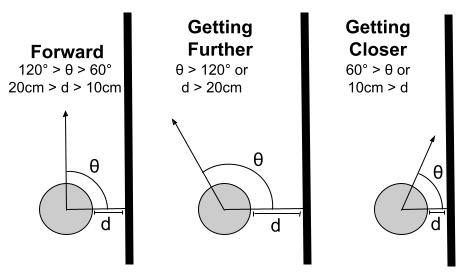
\includegraphics[scale=0.75]{images/Wall-Following Diagram.png}
    \caption{Three main courses of the robot}
    \label{Wall-following diagram}
\end{figure}

The course of the robot is determined by both an angle $\theta$ and a distance \textit{d}. Should the thresholds be exceeded, the robot will attempt to slowly return to the correct parameters. Since the robot considers the distance and angle, course adjustments should be minor and the robot should maintain a good distance from the wall. An example of an expected course adjustment is shown in the figure below.
\begin{figure}[H]
    \centering
    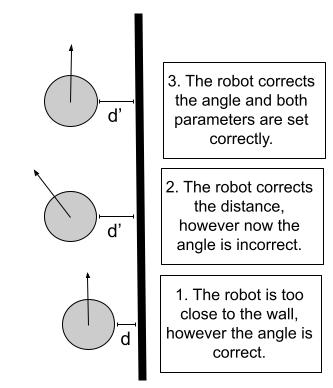
\includegraphics[scale=0.75]{images/Course adjustments.png}
    \caption{An example of a course adjustment}
    \label{Course Adjustments}
\end{figure}

The robot usually responds in a standard 3 step correction routine. The above figure describes a situation where the robot has slowly approached too closely to the wall. This is likely to happen occasionally, as the wheels are not perfectly aligned and it is difficult for the robot to achieve a perfect 90° angle with the wall. When this happens the robot will not exceed the angle threshold, but will eventually exceed the distance threshold. Then the following actions are taken:
\begin{enumerate}
    \item The robot has exceeded the distance threshold, but not the angle threshold.
    \item The robot turns left away from the wall slightly and until the distance is correct, but the angle is incorrect.
    \item The robot turns right to correct the angle. The  angle and distance are then correct and the robot returns to normal wall following behavior.
\end{enumerate}

\subsubsection{Robot Driver State Machine}
The robotDriver is a key node for robot navigation. It receives several events from three man nodes the IRSensor, Bumper and Captain. These events have several mutually exclusive values. They are expressed in the table below:

\begin{table}[H]
\centering
\caption{RobotDriver State Machine Events}
\label{State Machine Events}
\centering
\begin{tabular} { | p{3cm} | p{8cm} | p{3cm} | }
\hline
\textbf{Event} & \textbf{Values} & \textbf{Source Node} \\
\hline
Distance & TooFar, TooClose & IRSensor\\
\hline
Angle & Tight,Wide & IRSensor\\
\hline
Bumper & RPressed, LPressed, CPressed & Bumper\\
\hline
Captain Request & LTurn, RTurn, PassThrough & Captain \\
\hline
CounterTimeout & The state's counter has timed out. & RobotDriver\\
\hline
\end{tabular}
\end{table}%

The RobotDriver state machine has several actions that are largely a pair of linear and angular values that turn the wheels. The actions are described in the table below:
\begin{table}[H]
\centering
\caption{RobotDriver State Machine Actions}
\label{State Machine Actions}
\centering
\begin{tabular} { | p{3cm} | p{10cm} | }
\hline
\textbf{Action} & \textbf{Description} \\
\hline
Forward & Full forward movement. \\
\hline
Backward & Full reverse movement. \\
\hline
Right & No forward movement, full right movement. \\
\hline
Left & No forward movement, full left movement. \\
\hline
SLeft & Slight Left turn, forward and angular movement. \\
\hline
SRight & Slight Right turn, forward and angular movement. \\
\hline
CreepForward & Full forward at 1/4th speed.\\
\hline
\end{tabular}
\end{table}%

Using the input events and output actions the robot follows the logic of the RobotDriver state machine to navigate the tunnels.

The following is the state machine for the robotDriver which determines its internal logic.

\begin{figure}[H]
\caption{RobotDriver State Machine}
\centering
\hspace*{-2cm}
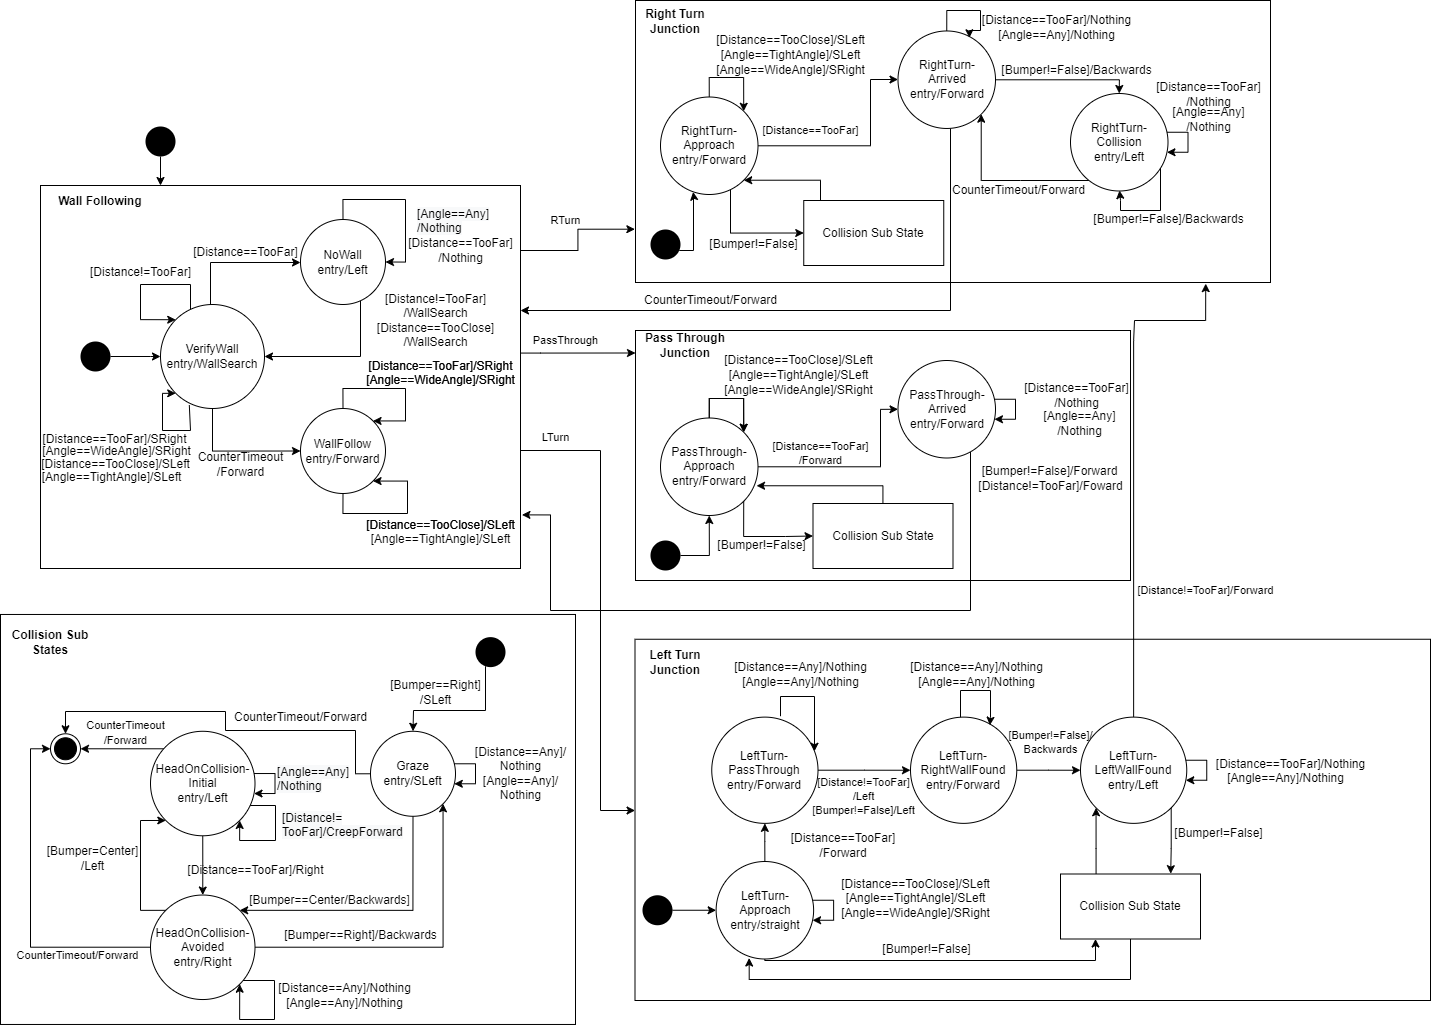
\includegraphics[scale=0.38]{images/RobotDriverStateMachine.png}
\centering
\end{figure}

\subsection{Junction Traversal in The State Machine}
\sectionAuthor{By Stephen Wicklund}

Junction traversals are states in the state machine which are triggered by events sent by the captain node. The captain node receives information from the beacons and determines which event should be sent to the robotDriver, i.e rightTurn.
\subsubsection{Right Turns}

\begin{figure}[H]
  \begin{subfigure}[b]{0.6\textwidth}
    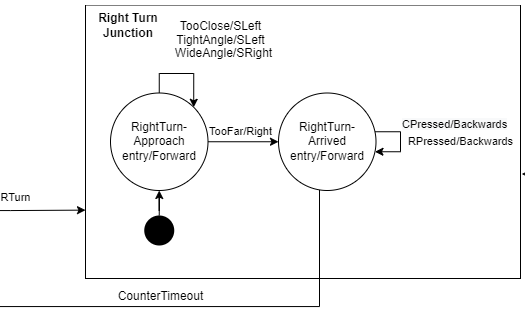
\includegraphics[width=\textwidth]{images/RightTurnZoomedIn.png}
    \caption{Right Turn states}
    \label{fig:f1}
  \end{subfigure}
  \hfill
  \begin{subfigure}[b]{0.5\textwidth}
    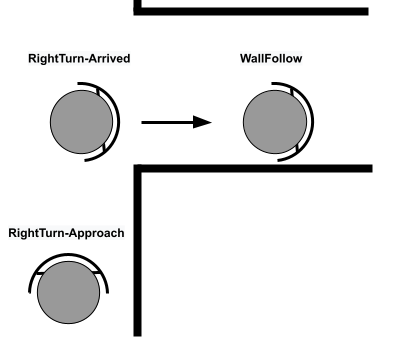
\includegraphics[width=\textwidth]{images/RightTurns.png}
    \caption{Right turn example}
    \label{fig:f2}
  \end{subfigure}
  \caption{Right turns states and example - Figure outdated}
\end{figure}

A right turn at a tunnel junction has a simple implementation composed of two states; RightTurn-Approach and RightTurn-Arrived. When the RTurn captainRequest is sent during the wall-following state the robot enters RightTurnApproach. This state continues to follow the wall on the right side and waits for the wall to no-longer be detected. During this state the robot can still make corrections to the wall-following, as these corrections are largely based on angle and not distance the robot can determine it is getting further from a wall with the angle and determine the wall is no longer there with the distance.

Once it is determined the wall is no longer to its right, the robot will enter the RightTurn-Arrived state. It will then perform a sharp 90\textdegree turn, a short forward movement, then transition to the WallFollow state.

If the robot fails to correctly detect the corner or attempts to turn too soon it will collide with the wall. This will trigger a special response to move further ahead, then reattempt the turn, it can repeatedly attempt this and will not attempt to wall follow until the bumper is no longer triggered after the turn.

\subsubsection{Pass Through}
\sectionAuthor{By Stephen Wicklund}

\begin{figure}[H]
  \begin{subfigure}[b]{0.6\textwidth}
    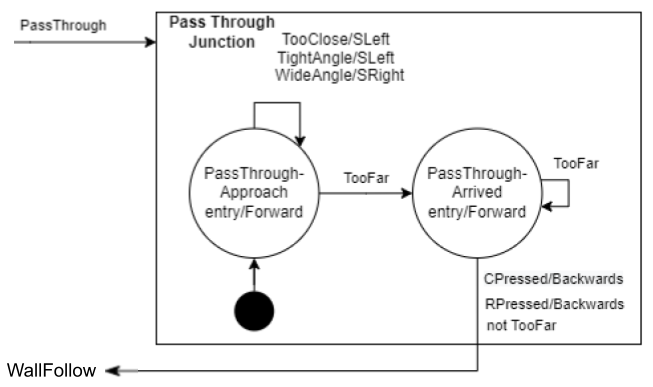
\includegraphics[width=\textwidth]{images/PassThroughStates.png}
    \caption{Pass through states}
    \label{fig:f3}
  \end{subfigure}
  \hfill
  \begin{subfigure}[b]{0.5\textwidth}
    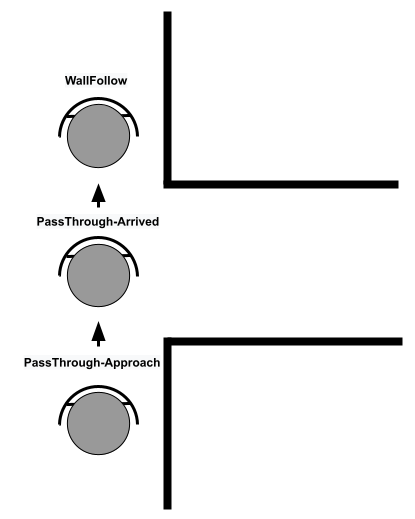
\includegraphics[width=\textwidth]{images/Pass Through Example.png}
    \caption{Pass through example}
    \label{fig:f4}
  \end{subfigure}
  \caption{Pass Through states and example - Figure outdated}
\end{figure}
Passing through a junction works very similarly to turning right. The robot enters a approach state and follows the wall until it can no longer be detected, adjustments can still be made based on angles though. Then once the wall is no longer detected, the robot continues straight until a wall is detected by either the IR sensors or by hitting the wall, then it re-enters the wall-following state.

The diagram below illustrates potential issues during a pass-through:
\begin{figure}[H]
    \centering
    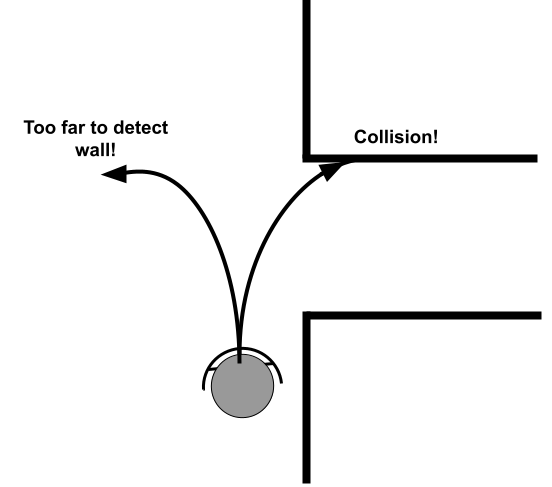
\includegraphics[scale=0.5]{images/Pass Through Issues.png}
    \caption{Potential issues during a pass-through}
    \label{Pass through issues}
\end{figure}

The robot may either drift too far right and hit the wall in the junction or too far left and not be able to detect the wall after it passes the junction. There are measures in place to prevent both these issues. If the robot collides with the wall it will hit the bumper and then avoid the corner as if it were an obstacle as outlined in the collision response section \ref{Collision Reponse}. If the robot drifts too far left it will time out and re-enter the wall following state, the robot will then look for walls to the right and eventually detect or collide with the wall and re-enter wall following.

\subsubsection{Left Turn}
\sectionAuthor{By Stephen Wicklund}

\begin{figure}[H]
  \begin{subfigure}[b]{0.55\textwidth}
    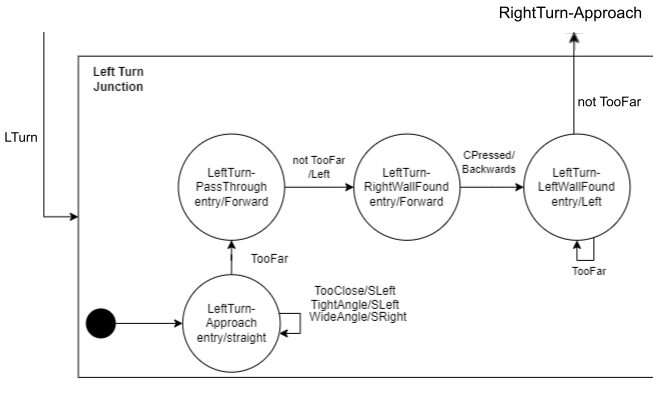
\includegraphics[width=\textwidth]{images/LeftTurnStates.png}
    \caption{Left Turn states}
    \label{fig:f5}
  \end{subfigure}
  \hfill
  \begin{subfigure}[b]{0.4\textwidth}
    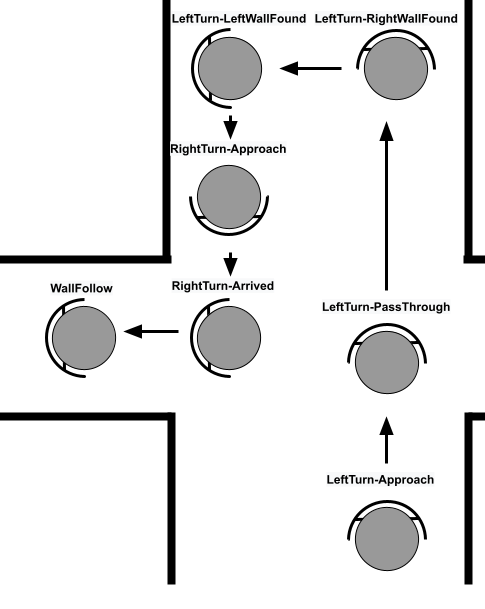
\includegraphics[width=\textwidth]{images/Left Turns.png}
    \caption{Left Turn example}
    \label{fig:f6}
  \end{subfigure}
  \caption{Left Turn states and example - Figure outdated}
\end{figure}

Left turns are the most complex junction traversal and also the most risky. To mediate this risk a left turn is a combination of a pass through, hall traversal and a right turn. This is implemented through four new left turn states. The full process of a left turn requires the following steps:
\begin{enumerate}
    \item The robot receives the LTurn event and transitions into the LeftTurn-Approach state.
    \item Once the wall is no longer detected, it transistions into LeftTurn-PassThrough. This behaves exactly like the Pass Through junction traversal.
    \item When the right wall is detected the robot transitions to the LeftTurn-RightWallFound state. The robot then turns left and crosses the hallway.
    \item When the robot collides with the left wall, it transitions into the LeftTurn-LeftWallFound state. It turns right and begins a right turn around the wall.
\end{enumerate}

Once the robot is across the hallway and approaching the junction again it can follow the same behavior as a right turn.

\subsubsection{Collision Response} \label{Collision Reponse}
\sectionAuthor{By Stephen Wicklund}
When a bumperEvent occurs the robot was unable to or did not correctly avoid obstacles and has physically hit something. This requires a response in an attempt to navigate around the object and avoid getting stuck. The magnitude of the collisions will determine the response that the robot takes.

\begin{figure}[H]
    \centering
    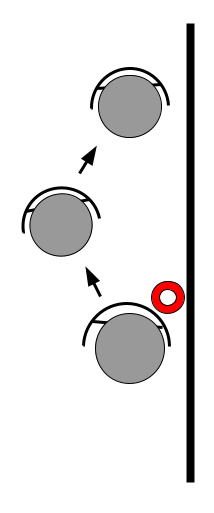
\includegraphics[scale=0.6]{images/Collision Response.png}
    \caption{Small Collision Response}
    \label{Small Collision}
\end{figure}

Small collision responses are characterized by only the right bumper activating. Small collisions will not stop the robot in its tracks and since it is round it can usually push past them. However, to avoid damaging the robot, it will steer to the left to avoid contact with the object as much as possible. As soon as the robot is no longer in contact with the object it can resume wall following. 

\begin{figure}[H]
    \centering
    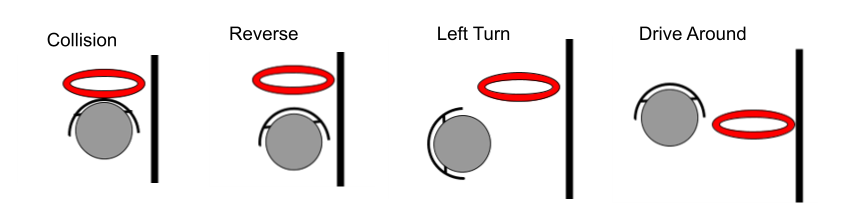
\includegraphics[scale=0.6]{images/LargeCollision.png}
    \caption{Large Collision Response}
    \label{Large Collision}
\end{figure}

Large collisions are characterized by both bumpers activating and require more attention to get around the object as the robot cannot drive past it without intervention. The robot will respond to these types of collisions with a multi-step process.

\begin{enumerate}
\itemsep0em 
    \item Reverse until the bumper is no longer active.
    \item Perform a left turn.
    \item Drive forward until the object is no longer detected with the wall-following sensors.
    \item Make a right turn and drive past the object.
\end{enumerate}

\subsection{Path Finding}
\sectionAuthor{By Emily Clarke}
With a map of the tunnel being turned into a graph with junctions as the vertexes and hallways as the edges, a graph search algorithm can be used to plot a path for the robots. There are two main options, a simple breadth first search (BFS) or Dijkstra's algorithm. In a breadth first search, the number of vertexes, or junctions, in the path are minimized. Using Dijkstra's, additional information about the distance between junctions can be used to minimize the distance traveled. 
BFS is the better choice as minimizing junctions is preferable to minimizing distance. This is because there is more that can go wrong during a junction traversal than simple wall following. An additional benefit is BFS is a simpler algorithm that is easier to implement and does not require knowing the distances of hallways between junctions.

\subsection{Scheduling Requests}
\sectionAuthor{By Stephen Wicklund}
\label{SchedulingRequests}
The scheduling of requests needs to consider two primary objectives; fairness and efficiency. The scheduling will also be decentralized as this improves scalability and allows the web server to operate as only a simple database handler.

To ensure that all requests eventually get assigned to a robot, requests will get aged after they've been created and have not been fulfilled for a specified period of time. When a request gets aged, its priority will increase by one level. This will ensure fairness in the scheduling scheme. This will be implemented in the database through the age and priority values. The age value is the time that the priority was increased last, these values are adjusted in a decentralized manner. When a robot searches for requests and determines that the age exceeds the aging time it will increase the priority and reset the age value to the current time.

To ensure that requests at an equal priority are given to the robot that is in the best position to handle that request we will use a decentralized bidding system. Idle robots periodically scan the database to determine if there are new requests that they may take. The robot then calculates the distance between itself and the pickup location of the request. It then inserts a `bid' for the closest request into the database, listing its robot ID along with its distance to the request, if the robot is the first bidder, it begins the bidding period and the expiry date for the bidding period is added to the database along with the bid. Robots then check to see if the bidding period has expired, once expired the robot with the smallest distance to the pickup location takes the request and all other robots return to bidding on other requests.

The request entry in the database is in the following format:
\begin{table}[H]
\centering
\caption{Database Request Table}
\centering
\begin{tabular} { | p{1.5cm} | p{1.5cm} | p{1.5cm} | p{2cm} | p{2cm} | p{3cm} | p{1.5cm} | }
\hline
Request ID & Age & Priority & Pickup Location & Destination Location & Bid \{RobotID, Distance\} & Bidding Expiry\\
\hline

\end{tabular}
\begin{tablenotes}
      \small
      \centering
      \item Note: Some columns which are not needed for scheduling have not been included.
\end{tablenotes}
\end{table}%


%=================================================================================
\clearpage
\subsection{Robot Power}
\label{RobotPower}
\sectionAuthor{By Emily Clarke}
A vital nonfunctional requirement to ensure project longevity is easy of setup and maintenance. In pursuit of this goal, electronics on top of the iRobot Create 2 should be powered solely by the iRobot Create's battery. This will greatly simplify power delivery and charging compared to alternatives such as a secondary battery pack.

\subsubsection{Power Requirements}
The power requirements for the two possible significant power draws are as follows:
\begin{description}
    \item[Raspberry Pi 4] The recommended power supply for a Raspberry Pi 4 is 5V at 3A\cite{Pi4Specs} for a total of 15W. This allows for at least 1A to go to attached sensors and accessories which is far more than any potential sensors this project will use.
    \item[Raspberry Pi Zero W] The Raspberry Pi Zero W uses a maximum of around 230mA at 5V (1.15W) during heavy loads and near half that for more typical loads \cite{PiZeroPower}.
\end{description}

\subsubsection{Power Sources}
The iRobot Create 2 can supply power in the following two ways. Note: this does not apply to the iRobot Create 1, our system design will assume an iRobot Create 2 but a non standard testing setup will be implemented on the iRobot Create 1. 
\begin{description}
    \item[Serial Port] The iRobot Create 2 has a serial port capable of providing 0.2A at 10V-20.5V for a maximum rated capacity of 2W \cite{BatterySpecs}. This serial port is constantly powered when the iRobot Create 2 is powered. 
    \item[Motor Driver] The iRobot Create 2 has several motor drivers, the main one capable of providing 1.45A at 12V for a maximum rated capacity of 17W \cite{BatterySpecs}. A 2.2mH 1.5A inductor is required to use the main motor driver.
\end{description}

\subsubsection{Power Plan}
The main motor driver with a rated capacity of 17W is more than capable of powering any electronics that could be implemented for this project. A simple buck converter circuit to bring the voltage down to 5v for the Raspberry Pi 4 can provide more amperage (3.4A) than the standard Pi 4 power supply (3A). This means that a Pi 4 powered via the motor driver can function as if plugged into the wall along with any sensors that work with a typical Pi 4 setup. The one drawback is that the main motor driver is not powered on boot until a command is sent over the serial cable. In order to use the motor driver to power the Pi 4, an additional lightweight controller is needed to run off the always powered serial port. This port provides more than enough power for a Raspberry Pi Zero W or similar micro-controller, although it is insufficient for the Pi 4. As with the motor driver, a simple buck converter circuit attached to the serial port provides more power (5V 400mA) than is needed to power the Pi Zero W (5V 230mA). The main purpose of the Pi Zero W is to run a boot sequence to power on the Pi 4 and from that point, the Pi 4 will be the primary controller.

%=================================================================================
%=================================================================================
\section{Web Interface}
\subsection{Front End}
\sectionAuthor{By Emily Clarke and Stephen Wicklund}
\label{FrontEndDesign}
The web application is the user interface for the entire mail delivery system. It should primarily allow users to:
\begin{itemize}
\itemsep0em 
\item Request a delivery robot
\item Make delivery requests
\item Monitor delivery requests
\end{itemize}

The web application should:
\begin{itemize}
\itemsep0em 
\item Look polished
\item Be intuitive to users
\item Be secure from malicious activity
\item Be available to users through any web browser
\item Function properly on a mobile device
\end{itemize}

A web framework such as Angular provides simple methods to achieve each of these requirements. For simplicity, this front end can also be hosted using a serverless web host such as Cloudflare Pages. See the back end section below for more information on serverless.

\subsection{Back End}
\sectionAuthor{By Emily Clarke}
The web application will run in conjunction with a serverless backend. Serverless does not mean there are no servers, but instead that a third party controls the low level server with easy access to the application running on top of it. This means there will be less to manage on the server side. It also ensures there aren't issues with out of date packages on a server operating system making replication difficult in the future. One downside is for easy replication, it relies on the chosen providers to still exist, but the market has matured enough to choose stable serverless providers. Going with a provider that does not use proprietary technology allowing for migration to other providers is ideal.

\subsubsection{Database}
The front end will receive data from a database. The backend will not have any active role so it will be implemented as simply as possible with a serverless database accessed via a http API. Since Cloudflare is already being used, their partner, Fauna, is a good, free choice for this. Fauna is primarily based on GraphQL which stores data in collections that are similar to SQL tables. The database model is defined in schema.gql and is as follows.

\begin{table}[H]
\centering
\caption{Database Model}
\label{databaseModel}
\centering
\begin{tabular} { | p{2cm} | p{5cm} | p{7cm} | }
\hline
Collection & Description & Fields \\
\hline
Beacon & Stores beacon information & id, junction, status*, paths \\
\hline
Junction & Stores junction information & id, beacons \\
\hline
Path & Stores map information & beacon, destBeacon, distance \\
\hline
Request & Stores requests & id, robot (id of robot handling request), timestamp, source, destination, sender, recipient, state*, age, bidExpiry, priority, bids: \{robot, distance\} \\
\hline
Robot & Stores robot information & id, location, status* \\
\hline
User & Stores user information & username, email \\
\hline
\end{tabular}
\begin{tablenotes}
      \small
      \centering
      \item Note: The entries for the first field in each collection are unique.
      \item Note: The last four Request fields, are detailed in \ref{SchedulingRequests} Scheduling Requests. 
      \item * values for these fields are explained in tables below
\end{tablenotes}
\end{table}%

\begin{table}[H]
\centering
\caption{Beacon$\rightarrow$Status}
\label{BeaconStatusTable}
\centering
\begin{tabular} { | p{2.5cm} | p{12cm} | }
\hline
Status& Description \\
\hline
Nominal & Beacon is charged and deployed. \\
\hline
BeaconFault & Beacon needs a new battery or other error. \\
\hline
InService & Beacon is not deployed. \\
\hline
\end{tabular}
\end{table}%

\begin{table}[H]
\centering
\caption{Request$\rightarrow$State}
\label{RequestStateTable}
\centering
\begin{tabular} { | p{2.5cm} | p{12cm} | }
\hline
State& Description \\
\hline
Pending & The request is waiting to be claimed by a robot. \\
\hline
InProgress & A robot is currently completing the request. \\
\hline
Completed & The delivery has been completed. \\
\hline
\end{tabular}
\end{table}%

\begin{table}[H]
\centering
\caption{Robot$\rightarrow$Status}
\label{RobotStatusTable}
\centering
\begin{tabular} { | p{2.5cm} | p{12cm} | }
\hline
Status& Description \\
\hline
Nominal & The robot is charged and available to complete a delivery. \\
\hline
InProgress & The robot is currently completing a delivery or recall request. \\
\hline
Charging & The robot is charging and is unable to complete a delivery request. \\
\hline
Stuck & The robot cannot continue normal operation. \\
\hline
InService & The robot is not deployed. \\
\hline
\end{tabular}
\end{table}%

\subsection{API and Communication}
\sectionAuthor{By Emily Clarke}
The API will be primary method of communication between the front end, database, and robots. With a serverless database such as Fauna, an http API is provided to access data. This API will be used to create the following specific API calls.

\begin{table}[H]
\centering
\caption{API Table}
\label{APITable}
\centering
\begin{tabular} { | p{3cm} | p{3.5cm} | p{4cm} | p{3cm} | }
\hline
Function & Description & Parameters & Server Response\\
\hline
Add Request & add request & \{``request": Request\} & Success or failure to add \\
\hline
Get Requests & Get requests from server & \{\} & A list of requests \\
\hline
Get Map & Get map from server & \{\} & The tunnel map \\
\hline
Update Request & Claim and update status of a request & \{``request": Request\} & Success or failure to update \\
\hline
Update Robot & Update robot status on server & \{``robot": Robot\}  & Success or failure to update \\
\hline
Update Beacon & Update beacon status on server & \{``beacon": Beacon\} & Success or failure to update \\
\hline
\end{tabular}
\begin{tablenotes}
      \small
      \centering
      \item Note: The fields for custom types are detailed above in Tables \ref{databaseModel}-\ref{RobotStatusTable}
\end{tablenotes}
\end{table}%

\subsubsection{Communication}
With the serverless approach, each robot will act as an independent client. Requesting and claiming requests on its own.

\begin{figure}[H]
\caption{Web Server Communication Sequence Diagram}
\centering
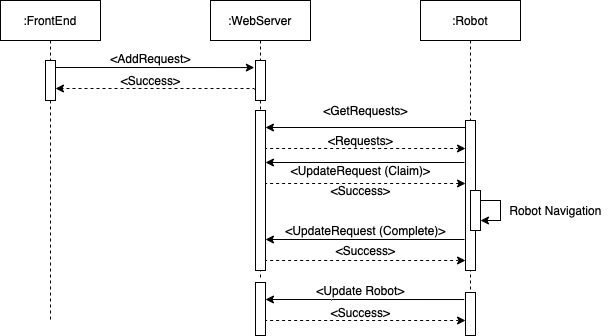
\includegraphics[scale=0.7]{images/CommunicationSequenceDiagram.png}
\centering
\end{figure}

The above figure first shows a request being submitted to the WebServer from the FrontEnd. The term WebServer refers to the serverless database. The robots will them get and claim requests. After navigating and executing the request, the robot will mark it as complete with UpdateRequest. With every API call, the WebServer will provide a response to indicate the message was successfully received.

%========================================================================================

\section{Instrumented Environment}
\sectionAuthor{By Emily Clarke}
The Bluetooth beacons are part of the positioning system for the mail delivery robot. They may not be the sole positioning method. The Bluetooth beacons should allow the robot to:
\begin{itemize}
\itemsep0em 
\item Determine a rough location along a path
\item Connect to the beacon from a reasonable distance
\item Check the battery level of the beacon
\end{itemize}

\subsection{Beacon Data Interpretation}
\sectionAuthor{By Stephen Wicklund}
\subsubsection{Identifying Beacons}
When the robot scans and detects a Bluetooth signal, it must then determine if this signal belongs to a beacon and which beacon. This is done by inspecting the MAC address of the Bluetooth signal and referring to the cached lookup table stored on the robot. A master lookup table exists on the web-server; however, as the robot rarely has access to the web-server it will cache this data internally and update it when it is able to. If the robot detects a Bluetooth signal for which the MAC address does not exist on the lookup table, it will ignore it. The lookup table contains the MAC address and identifying information about the junction that the robot is approaching for each Bluetooth beacon.

%%%%%%%%%%%%%%%%%%%%%%%%%%%%%%%%%%%%%%%%%%%%%%%%%%%%%%%%%%%%%%%%%%%%%%%%%%%%%%%%%%
\section{Autonomous Delivery Robot}
\subsection{Robot Operating System}
\sectionAuthor{By Stephen Wicklund}
\subsubsection{ROS2 Migration}
For the future of the project it was decided at the beginning of development that the project would be migrated from ROS Kinetic to ROS2 Foxy. Following suit the Raspberry Pi 4 will now be running Ubuntu 20.04 (previously ubuntu 16.05) and at least python 3.5 (previously python2.7).

This was done primarily to target python3.5 and to use a platform that was still being maintained, as ROS kinetic (along with Ubuntu 16.04) had reached its end of life April, 2021. With this migration newer python3.5 libraries can be used, and the risk of relying on deprecated libraries which are buggy or broken is reduced. ROS2 Foxy also supports more and newer operating systems, including ubuntu 20.04 which this project will target. Newer tools, libraries and other software will likely target ROS2 and more recent ubuntu distributions which will benefit the future of the project.

The migration did not require extensive work as there were only a handful of scripts being re-used. To migrate these scripts to ROS2, they had to be written in python3.5, then the node structure rewritten. The node structure is only a few lines of code dictating which topics the node subscribes and publishes to. This is simplified in ROS2 as nodes inherent from a Node class and much of the logic is handled behind the scenes. Furthermore, the create\_autonomy ROS library has already been migrated to ROS2.

\subsubsection{Current ROS Node Map}
\begin{figure}[H]
    \centering
    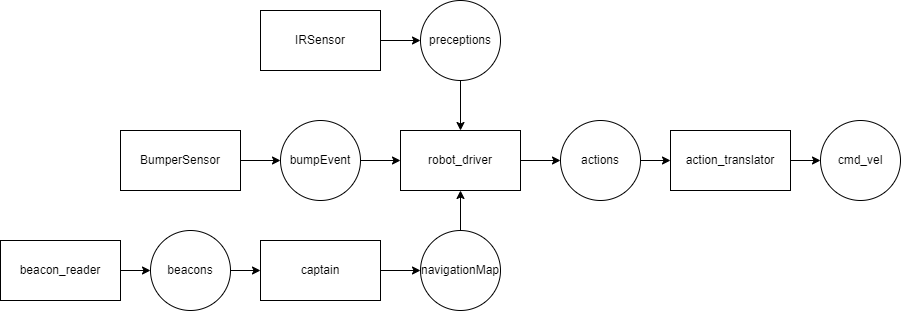
\includegraphics[scale=0.5]{images/ROS Node Diagram.png}
    \caption{Current ROS Node Map}
    \label{Current ROS Node Map}
\end{figure}

The above diagram shows the current flow of information for the implemented ROS nodes. Nodes are indicated with rectangles and topics with circles.

The \textit{robot\_driver} is the central node for the navigation system, it subscribes to topics which contain key navigational information and publishes the actions that the robot must then perform. The \textit{action\_translator} converts the published actions to forward and angular velocities published in the \textit{cmd\_vel} topic, which are read by \textit{create\_autonomy} to drive the robot.

The \textit{IRSensor} node reads and processes the information from the infrared  sensors to get a angle and distance which is then published to the perceptions topic. The \textit{BumperSensor} node reads the bumper and publishes to the bumpEvent node when appropriate. The \textit{beacon\_reader} node reads raw Bluetooth data and publishes only the data which corresponds to the MAC address of beacons in the database to the beacons topic. The \textit{captain} node tracks nearby beacons and publishes navigational events to the navigationalMap topic, currently only docking/undocking are implemented, but these events will include turns and other navigational state changes.

\subsection{Wall-Following Navigation}
\sectionAuthor{By Stephen Wicklund}
\subsubsection{State Machine Implementation }
The state machine is implemented as a node in python using the following two classes.

\begin{python}
class DriverStateMachine:
    def __init__(self, initialState):
        self.currentState = initialState
    def run(self, distance,angle,captainRequest):
        return self.currentState.run(distance,angle)
    def next(self,distance,angle,captainRequest):
        self.currentState = self.currentState.next(distance,angle,captainRequest)
\end{python}
The DriverStateMachine class stores our current state and runs our state machine. The next function used to determine the next state is called every time a input is changed (distance, angle or captainRequest). On a 2Hz timer the robotDriver calls the run function of the current state which returns the action that should be taken.

\begin{python}
class DriverState:
    counter = 0
    def run(self):
        assert 0, "Must be implemented"
    def next(self, distance,angle,captainRequest):
        assert 0, "Must be implemented"
    def toString(self):
        return ""
\end{python}

The DriverState class is inherited by all states. Each state has a run function that is executed when it is the current state and a next function that determines which state it should transition to each tick. The counter is a static variable that is used by states to keep track of how many ticks they've been active and is used in some states to timeout when they've been in their state for a specific amount of ticks.



\subsubsection{Captain}
The captain node subscribes to beacon data and publishes captain requests primarily to the robotDriver.
\begin{figure}[H]
    \centering
    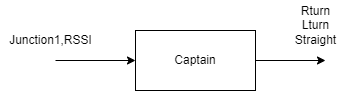
\includegraphics[scale=0.75]{images/CaptainCloseUp.drawio.png}
    \caption{The inputs and outputs of the captain node.}
    \label{Captain Node Closeup}
\end{figure}

Each individual data-point cannot give a indication on whether a beacon has been passed by the robot or not. Therefore the captain collects the last 5 data points, averages them, collects 5 more data points, averages them, then creates a slope between the two averages. Outliers are discarded to not affect the averages. The slopes are tracked over time and when a sign change occurs this is an indication that the robot has passed the beacon and it responds. 

\begin{figure}[H]
    \centering
    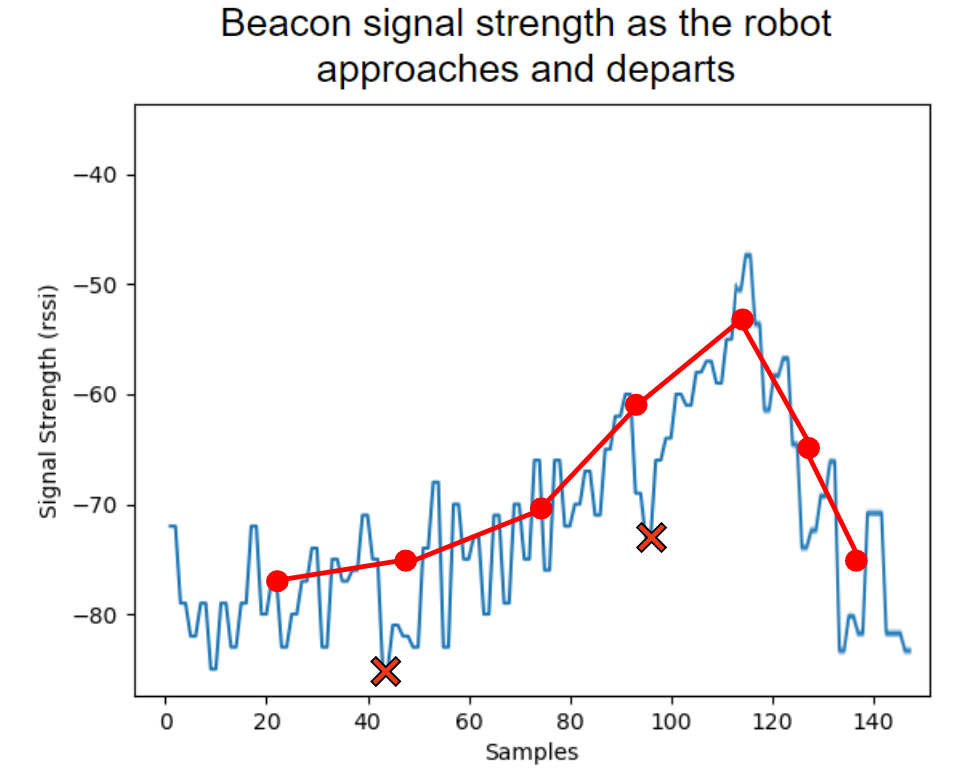
\includegraphics[scale=0.4]{images/CaptainDataAnalysis.png}
    \caption{Averages and slopes overlaid over the signal strength recorded from the robot.}
    \label{Captain Node Data Analysis}
\end{figure}

The above figure shows how the captain node determines that a beacon has been passed. Red dots indicate averages and red lines the slopes. Outliers are removed and are shown as crossed out data points. When the slope changes from positive to negative for two slopes, it will confirm that a beacon has been passed.

Once the captain determines the robot has passed a beacon, it determines the proper course of action and publishes it to the robotDriver which causes a state change to respond to the upcoming junction accordingly. (Currently only right turn).

\subsubsection{Bumper}
\sectionAuthor{By Stephen Wicklund}
Both the iRobot Create 1 and Create 2 have a front bumper that can detect collisions with objects. The bumper works by having two levers that when pressed trigger a Boolean that can be read through the create\_autonomy library. The mechanics of the bumper allow for only the left or right lever to be pressed at a time, and when the center is pressed both levers get pressed.
\begin{figure}[H]
    \centering
    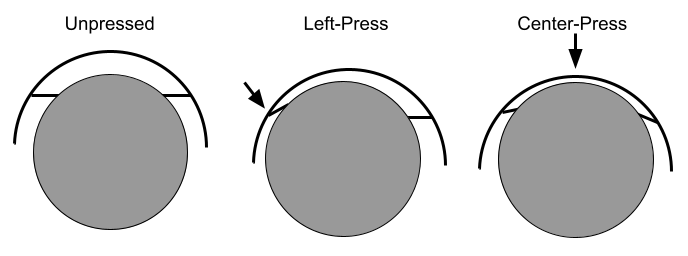
\includegraphics[scale=0.5]{images/Bumper Presses.png}
    \caption{Different actions on the robot bumper}
    \label{Robot Bumper Actions}
\end{figure}

The iRobot Create 2 has additional features in the bumper that allow it to detect light. The create\_autonomy library resolves these differences in hardware and publishes the same bumper object. On the iRobot Create 1, since there are no light detectors these values are always false or 0.  

Below is an example of a bumper object from the iRobot Create 1:
\begin{python}
is_left_pressed: False
is_right_pressed: False
is_light_left: False
is_light_front_left: False
is_light_center_left: False
is_light_center_right: False
is_light_front_right: False
light_signal_left: false 0
light_signal_front_left: 0
light_signal_center_left: 0
light_signal_center_right: 0
light_signal_front_right: 0
light_signal_right: 0
\end{python}

The bumperSensor node sits in between create\_autonomy and the robotDriver. It reads the bumper objects that are published from create\_autonomy and publishes four simple states: 'unpressed', 'Lpressed', 'Rpressed' or 'Cpressed' for Left, Right and Center presses respectively.

\subsubsection{Collision Response}
\sectionAuthor{By Stephen Wicklund}
The robot responds to collisions in two ways as outlined in section \ref{Collision Reponse}; small collisions and large collisions. Small collisions are implemented with one simple state which causes the robot to back up, turn slightly left, then resume wall-following. 

Large collisions are implemented as two states; HeadOnCollisionAvoid and HeadOnCollisionReturn. The robot first avoids the obstacle by backing up, then turning left and following the object. When the robot no longer detects the object, it enters the HeadOnCOllisionReturn state and attempts to return to wall following. In some cases the robot can make a head-on collision with the wall it is following, in this case the robot follows the object, the object maintains within the threshold distance for a period, then the robot begins following the object (a wall).

When colliding with a large object the robot will respond as shown below:
\begin{figure}[H]
    \centering
    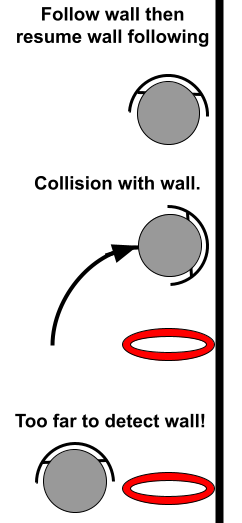
\includegraphics[scale=0.5]{images/BigCollisionExample.png}
    \caption{An example of a large collision}
    \label{Large Collision Issues}
\end{figure}

After the robot navigates around a large object it is often too far to find the wall safely. The robot then turns right in a circle and eventually collides with the wall. It can then re-enter the HeadOnCollisionAvoid state and when the wall does not end it resumes wall-following.

\subsection{Per-Robot Variable Tuning}
\sectionAuthor{By Emily Clarke}
Since every robot is manufactured with variations, or has wear, hard-coded behaviour is not consistent. This is further exasperated by using two different model years of the Create robot. For this reason, it is advantageous to be able to easily adjust any hard-coded parameters on a robot by robot basis. All hard-coded parameters in the code base have been pulled into a dictionary called tuningConstants. This dictionary contains default values for any such constant.

In order to allow for easy tuning, every script that uses tuningConstants checks for per-robot overrides in the following file: /var/local/magicNumbers.csv. If a specific value is listed in this file, it gets overridden, if it is absent, the default is used. The csv file is not necessary if only default values are desired.

Since this override check happens at run time, tuning the values is not only simple, but also can be done as part of a admin robot setup process without needing to recompile the software for each robot. This is also advantageous for development since constants can rapidly be tuned without recompiling.

Initial tests at tuning robots has resulted in improved visually perceived performance. More tuning is necessary for ideal performance on both robots. This new tuning process is far easier to keep track of than previous attempts.

\subsection{Path Finding}
\sectionAuthor{By Emily Clarke}
To put all of the ROS pieces together, the robot must now be able to determine how to get from point A to point B; the mail sender to the recipient. The following map is annotated with initial locations of beacons and junction IDs. A subsection of the tunnels has been chosen consisting of everything South and West of Minto Building. One important thing to note is that the directions listed on the map are to signify the frame of reference for each section of the tunnels and are not necessarily true cardinal directions.

\begin{figure}[H]
    \centering
    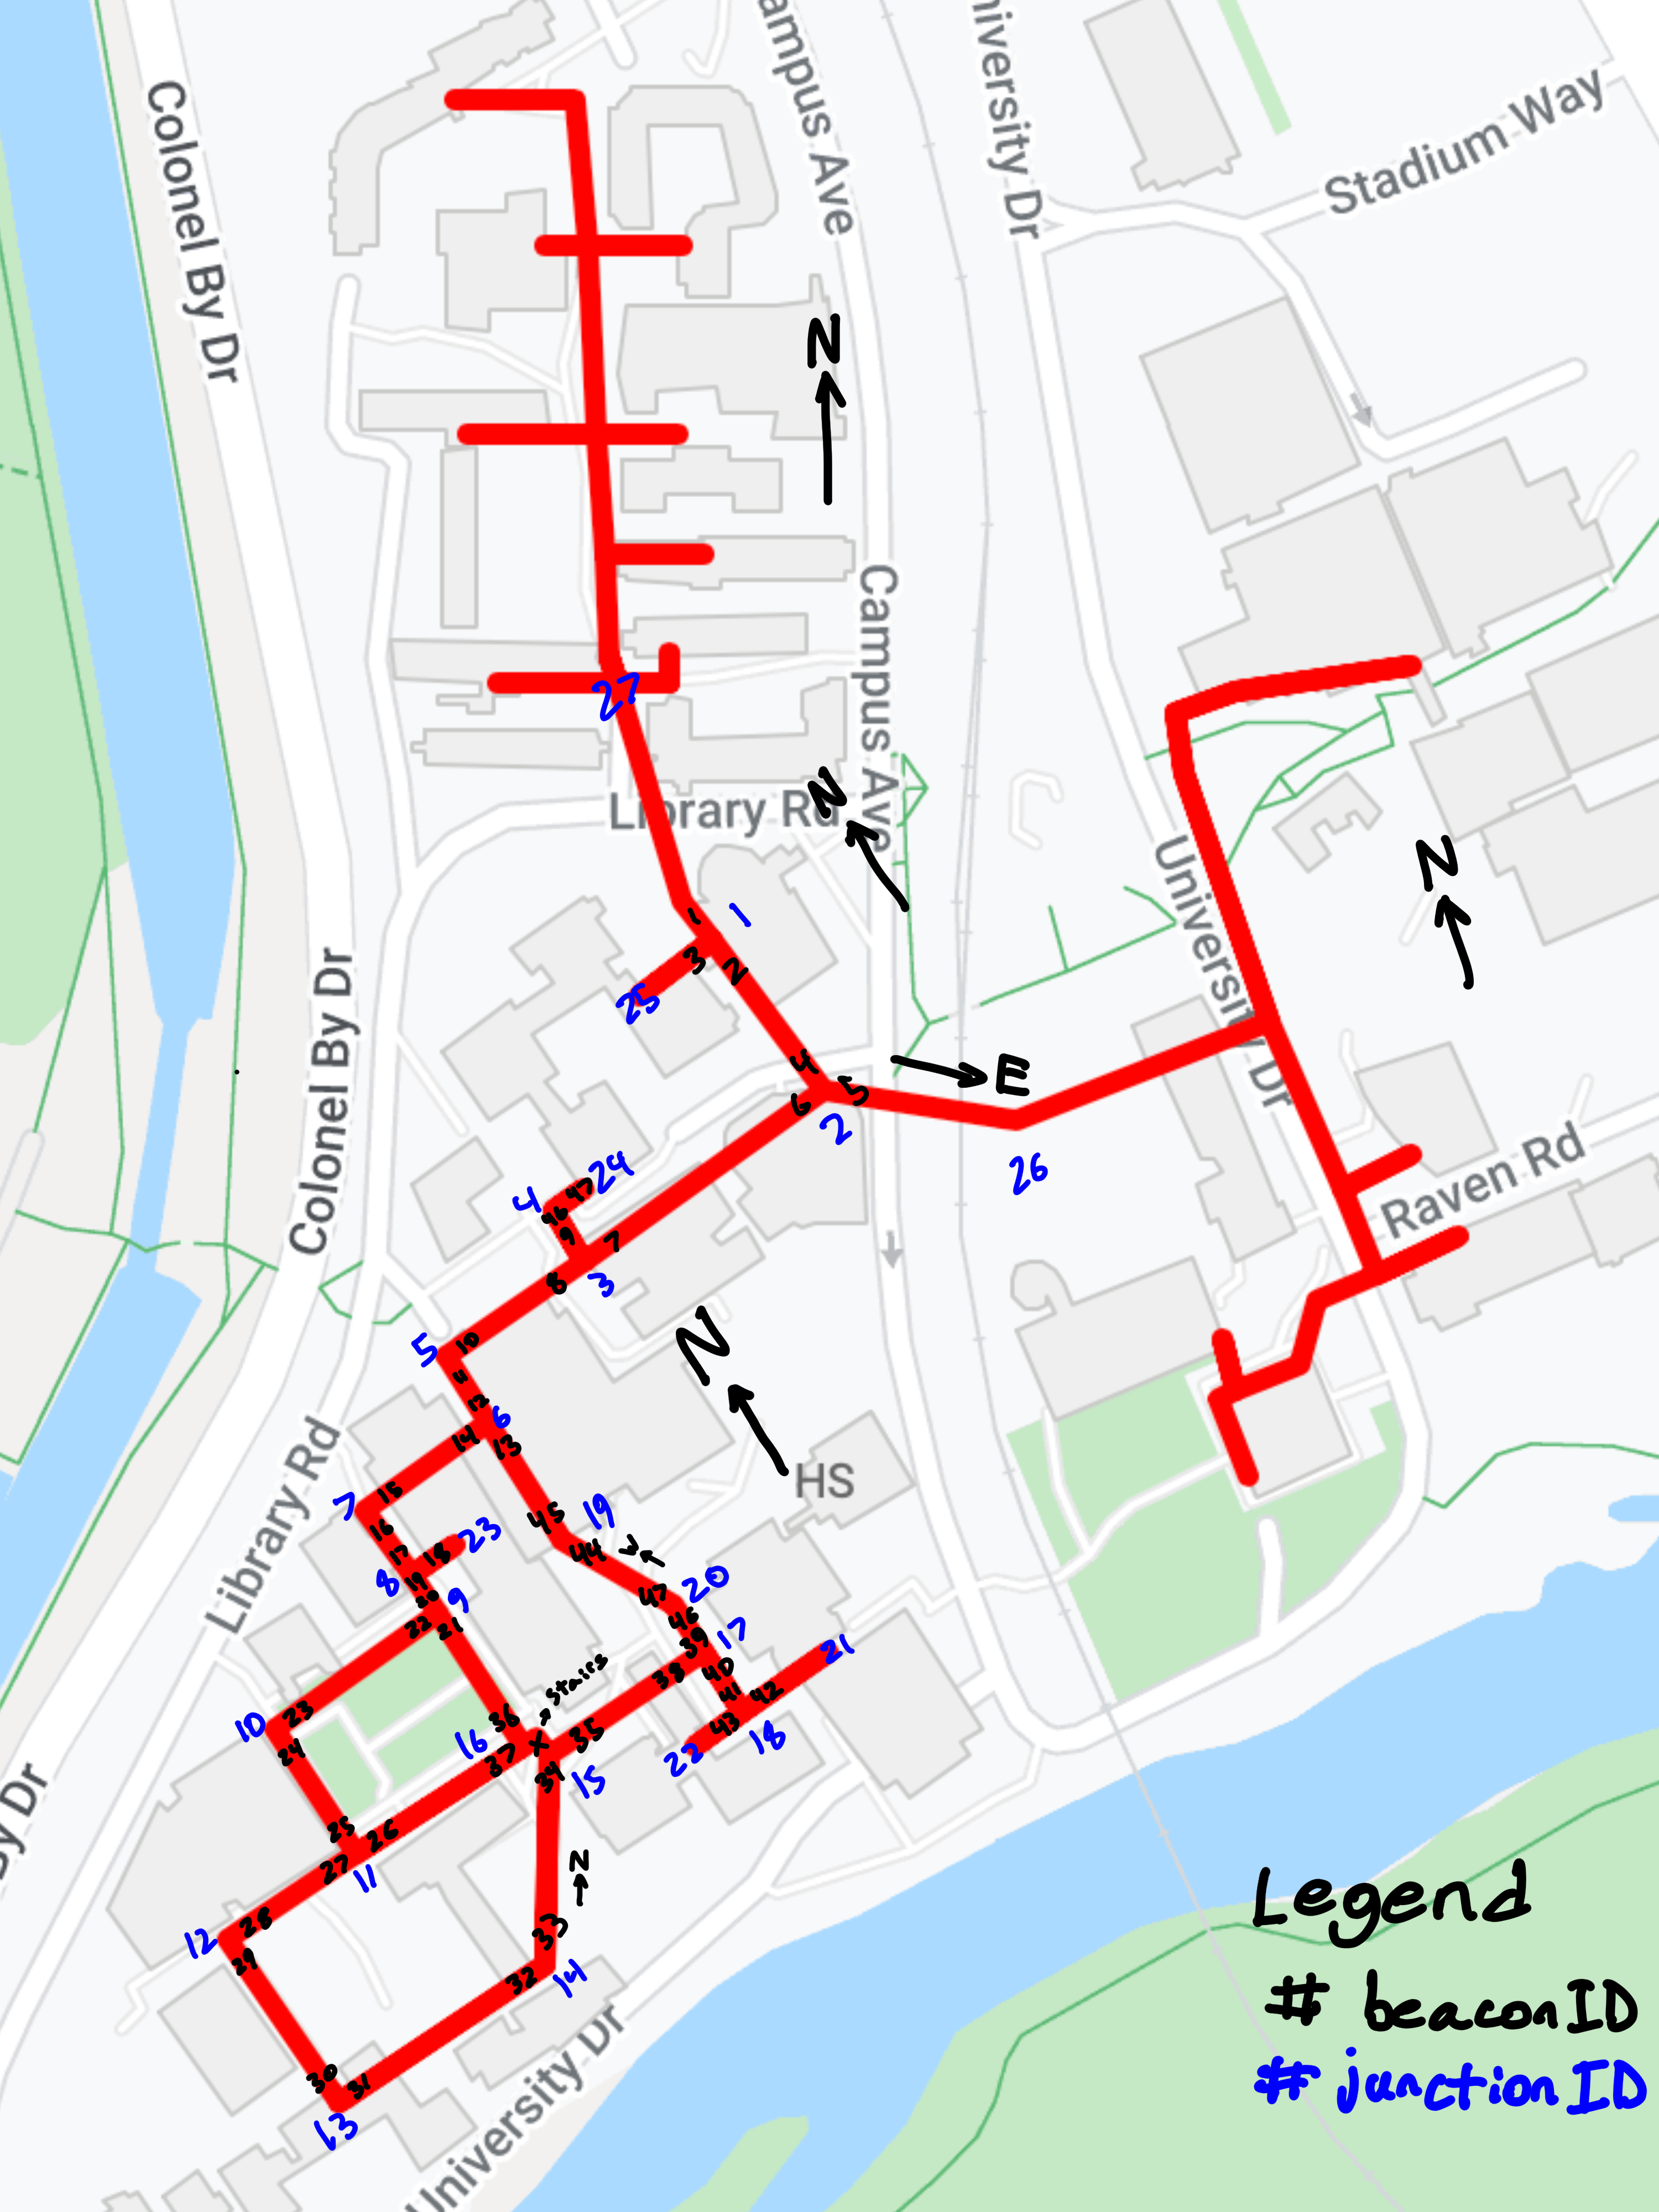
\includegraphics[scale=0.4]{images/map.png}
    \caption{Beacon and Junction IDs of Carleton Tunnels}
    \label{IDmap}
\end{figure}

Each robot stores this map in a CSV file using the following format:

\begin{table}[H]
\centering
\caption{Map Table}
\centering
\begin{tabular} { | p{1.5cm} | p{3cm} | p{3cm} | p{3cm} | p{3cm} | }
\hline
Junction ID & North & East & South & West\\
& \{Beacon ID, & \{Beacon ID, & \{Beacon ID, & \{Beacon ID, \\
&DestJunction\}&DestJunction\}&DestJunction\}&DestJunction\}\\
\hline
\end{tabular}
\end{table}%

The map is stored as a graph with junctions as vertexes and the tunnels as edges. Each junction has some set of edges coming out of it assigned to North, East, South, or West. An example of this file based on Figure \ref{IDmap} exists as map.csv.

\subsubsection{Path Finding Algorithm}
To determine how to navigate from point A to B, a Breadth First Search (BFS) is implemented on the graph. Below is the output of the algorithm determining the necessary path and turns to go from Junction 1 to Junction 13 on the map.

\begin{figure}[H]
    \centering
    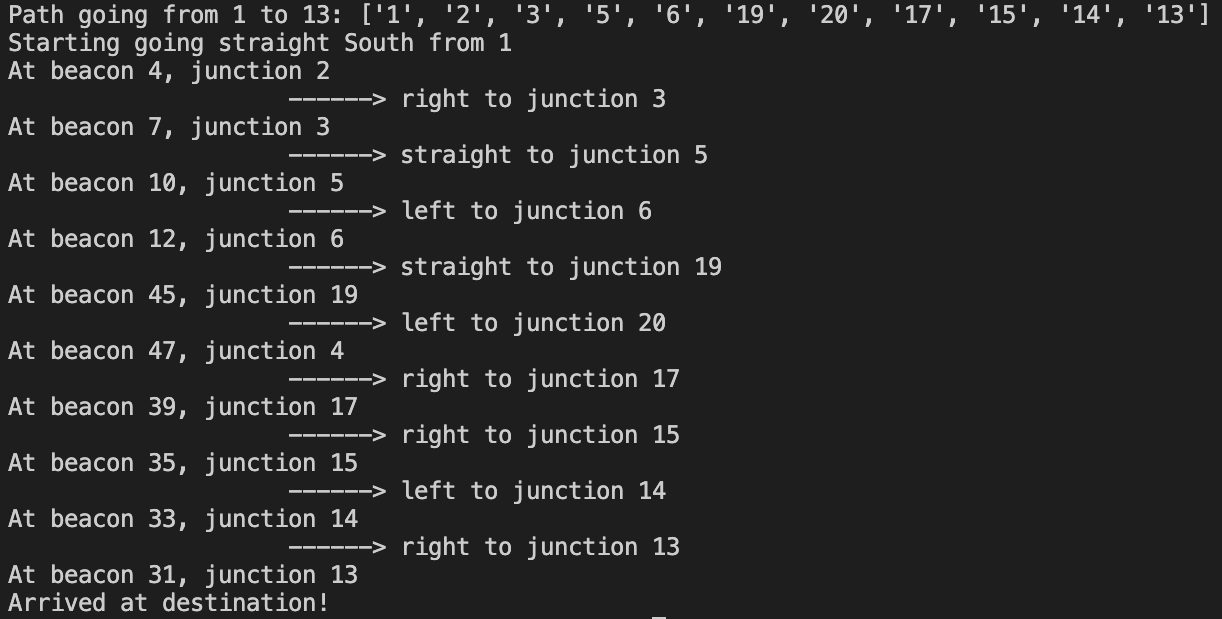
\includegraphics[scale=0.33]{images/pathfinding.png}
    \caption{Path finding example output}
\end{figure}

The methods that make up this algorithm are explained in more detail below.

\subsubsection{Methods}
In addition to the BFS graph search, pathFind.py also implements additional methods. The first allows a robot to determine which junction it is at based on a nearby beaconID. Another allows the robot to determine what beacon it should expect to encounter when approaching an intersection. This method could be used to implement error checking. Finally, there is a method to determine what direction to turn at a junction to get to the next target junction. All of these methods can be combined into a generic path finding algorithm which is outlined below in pseudocode.

\begin{python}
# when encountering a beacon, curBeacon -> determine junction
curJunc = beaconToJunction(curBeacon)
# determine path to known target destJunc using BFS
path = bfs(curJunc,destJunc)
# determine necessary turn at the current junction
turn = findTurn(curBeacon,path[0])
# repeat above and break when curJunc = destJunc
\end{python}

Even if the robot makes a wrong turn and ends up at an unplanned junction, this algorithm will update the path and eventually arrive at the desired destination.

\section{Web Interface}
\subsection{Front End}
\label{webInterfaceImplementation}
\sectionAuthor{By Emily Clarke}
An example front end has been implemented which can display a list of delivery requests from an array sourced from a simulated http request. There is also a form to submit a new request and then the message gets sent in a simulated http request and logged to the screen. This front end can hook into the back end with the addition of API calls. Approximately half of the code to implement the API calls has been written.

This falls short of the requirements outlined in the front end design section (\ref{FrontEndDesign}) although continuing development was deemed out of scope for this year.

\subsubsection{Angular}
The example front end was built using Angular, a typescript-based web application framework. Angular is only one possible framework that meets the requirements.
\begin{description}
   \item[PWA] Angular allows for the creation of progressive web apps (PWA) which are applications delivered through the web but intended to deliver app-like experiences across any platform.
   \item[Code Generation] Angular has many tools for code generation, allowing for rapid creation of polished looking interfaces.
   \item[Templates] Angular has a powerful template syntax which allows for creation of complex UIs without having to reinvent the wheel at every step.
\end{description}
The primary reason for choosing Angular specifically is prior experience with the framework. 

\subsubsection{Serving Front End}
The Angular front end was planned to be served using Cloudflare Pages. Cloudflare Pages is a free website hosting option for with no limits that constrain our project. Using Cloudflare Pages eliminates the need to manage a web server and can simply display the Javascript exported from Angular. The Angular code is independent of Cloudflare and could be deployed anywhere that supports serving Angular.

The example front end has not deployed on Cloudflare pages and has only been run locally from a terminal.

\subsection{Back End}
\sectionAuthor{By Emily Clarke}
A serverless database has been set up using Fauna. Fauna databases can be accessed using GraphQL queries and are organized into collections. The schema for the database is described in the schema.gql file. The following collections have been implemented:
\begin{itemize}
\itemsep0em 
\item Request - Information about delivery requests
\item User - User information
\item Robot - Robot status and location
\item Path - Map routes
\item Junction - Information about tunnel junctions
\item Beacon - Information about beacons
\end{itemize}

The schema.gql file allows for this database to be easily recreated in Fauna or another similar GraphQL database provider by uploading the file.

\subsection{API and Communication}
\sectionAuthor{By Emily Clarke}
API calls have been created as Python functions for easy integration into ROS. These methods are contained in the api.py file and can be used if this file is imported into a ROS script. The functions the robots will mainly use are outlined in the below table although additional functions exist in the file. Integration of the API into ROS was not completed.

\begin{table}[H]
\centering
\caption{Implemented API Table}
\label{ImpAPITable}
\centering
\begin{tabular} { | p{3cm} | p{3.5cm} | p{4cm} | p{3cm} | }
\hline
Function & Description & Parameters & Server Response\\
\hline
getRequests & Get all requests from server & \{\} & A list of requests \\
\hline
getOpenRequests & Get available requests from server & \{\} & A list of requests \\
\hline
claimRequest & Claim and update status of a request & \{``requestID": int, ``robotID": int\} & Success or failure to update \\
\hline
completeRequest & Mark request as completed & \{``requestID": int\} & Success or failure to update \\
\hline
updateRobot & Update robot status on server & \{``robotID": int, ``status": String, ``location": String\}  & Success or failure to update \\
\hline
updateBeacon Status & Update beacon status on server & \{``beaconID": int, ``status": String\} & Success or failure to update \\
\hline
getMap & Get map from server (incomplete) & \{\} & The tunnel map \\
\hline
\end{tabular}
\begin{tablenotes}
      \small
      \centering
      \item Note: The state and status values can be found in Tables \ref{BeaconStatusTable}-\ref{RobotStatusTable} in the design chapter
\end{tablenotes}
\end{table}%

The response to each api command will return the updated database entry. From this response, success or failure can be determined. 
GraphQL has an automatic ID for data entries accessed using \_id. Current implementations for all IDs use this automatic ID.

\subsubsection{getMap}
The api method to automatically build the local robot map file was not  completed. In the GitHub, map.csv holds the example map for the Carleton tunnels and can be loaded onto the robot manually. 

\subsubsection{Front End Communication}
Since the example front end is implemented using Angular, it cannot use the api.py file. The api.py file must be translated to typescript for use. 

\subsubsection{Claiming Requests}
Since robots can claim requests independently, a race condition can arise. The simplest solution to this is to wait a time, such as thirty seconds, after claiming a request and verifying that no other robot has overridden it. If the robot's ID is still listed on the request, that robot can fulfill the request. If another robot claimed it at the same time and is listed, that other robot will fulfill it.


% \section{Progress \& Future Work}

% \subsection{Project management}
% \subsubsection{Adherence to procedures}
% \sectionAuthor{By Emily Clarke}
% In our proposal we outlined a number of procedures to aid in agile programming. While some aspects have been quite successful, notably continuous integration to ensure pieces work together consistently, others have been less so. At this point, the code review has broken down due to a number of external factors that were not adequately planned for. Going forward, a strong effort needs to be made to correct course in order for the project to have a successful outcome.
% \subsubsection{Timeline}
% \sectionAuthor{By Stephen Wicklund}
% According to the timeline in section \ref{timeline}, the project should currently be at the stage of \textit{basic robot autonomy}. Which as described in the report;
% ``The robot responds to requests submitted from the web application autonomously.  The robot can follow a wall.  The robot can determine which beacons are nearby."

% Currently the robot can follow a wall and can determine which beacons are nearby. However, the web application and database have not been integrated with the robot currently and requests cannot be submitted and sent to the robot. We believe there is less than a week of work to achieve this final goal and the risk of issues or further missing this deadline is low as there are few unknowns.

% The next milestone is \textit{Intermediate Robot Autonomy} and is slated to be complete February 31st. Which as described in the report; ``The robot can receive requests and attempt to navigate to them without assistance, including through intersections. The web application looks functional and is intuitive."

% We believe that there is a high likelihood that this deadline will be met. All of the inputs have been tested and the basic state machine is implemented. Further development will focus on navigating intersections and junctions which is a continuation of the work already done and will have less unknowns. Following the schedule during this time work will also be done to improve the web application.

% \subsection{Future plans}
% \sectionAuthor{By Emily Clarke}
% Our primary focus is creating an interesting project which is centered around the robot. For this reason, we will first be focusing on basics and then expanding on as time allows. The request bidding system outlined in section \ref{SchedulingRequests} will only be implemented if there is extra time. We believe we are still on track to complete the important requirements outlined in the proposal.
\chapter{Testing \& Evaluation}
\section{Autonomous Delivery Robot}
\subsection{ROS Stub Testing}
\sectionAuthor{By Emily Clarke}
Due to the publisher subscriber architecture of ROS, stub testing is very easy to implement. Stub testing is when artificial inputs to nodes are provided to observe the behaviour in a controlled way. A simple bash or Python script can be written to publish arbitrary data to the ROS topics on a timed schedule. Using this, any of nodes can be tested individually. For example, the state machine could be tested with predefined sensor readings without needing to have the robot operational. In depth stub testing is highly recommended for any future development.

\subsection{Navigation Analysis}
\sectionAuthor{By Stephen Wicklund}
The robot navigation process is complex with various input and outputs that are changing constantly. As complexity is added to the navigation process it becomes increasingly difficult to debug and analyze what the robot is seeing and how it is responding to these inputs. In order to better understand the robot, tools were created to visualize the inner mechanisms of the robot.

\begin{figure}[H]
    \centering
    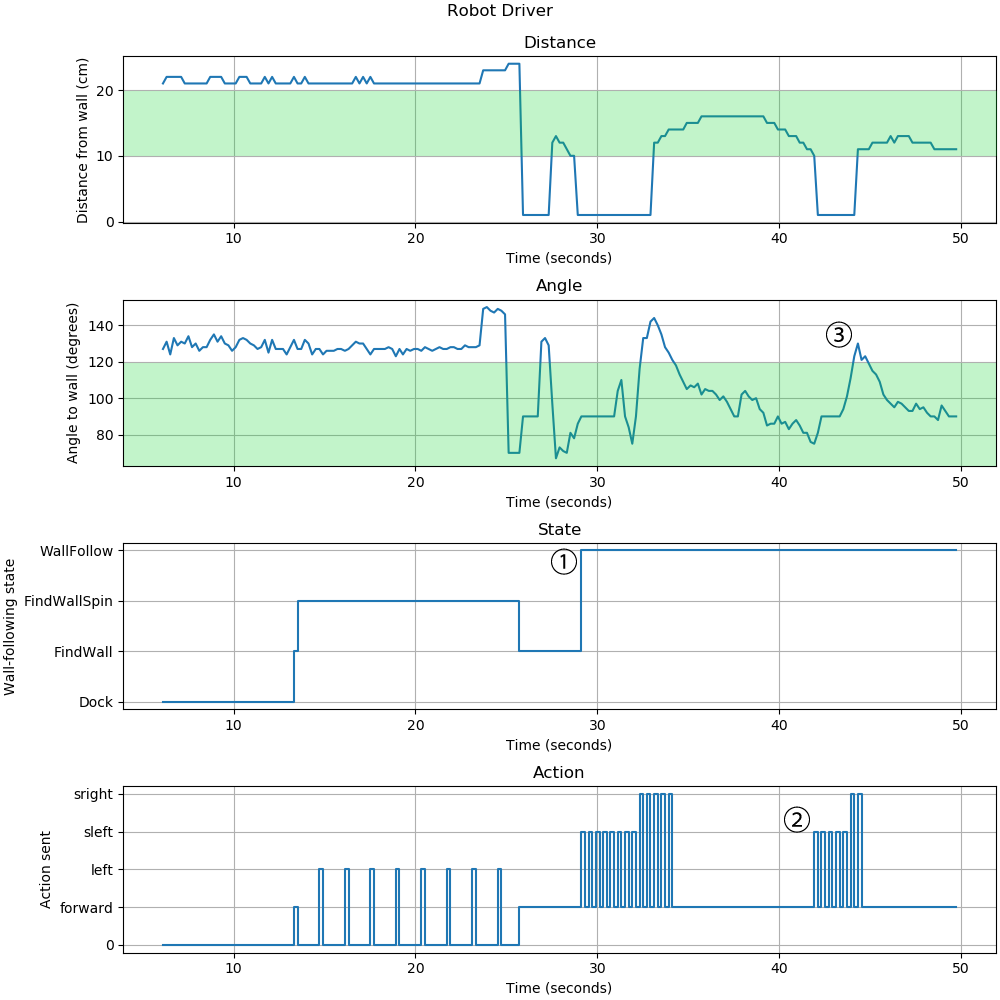
\includegraphics[scale=0.6]{images/driverPlotAnnotated.png}
    \caption{An example of the robot driver states, inputs and outputs as it finds and follows a wall}
    \label{Robot Driver Plot}
\end{figure}

The above figures shows an example of the output of our data analysis. It tracks the inputs of the IR sensors, the distance and the angle as well as the current state and the output action. The x axis shows the elapsed time since the robot began operation. It should be noted that the actions are sent continuously at a rate of 2Hz. Anytime the robot is not performing and being sent an action, the action sent will be 0.

At marker \#1 in figure 11 the robot transitions into the WallFollow state, this indicates that a wall has been detected and the robot will begin following it. After this marker the robot will make minor course adjustments to get the angle and distance measurements within the thresholds. The thresholds are the value ranges highlighted in green.

At marker \#2 the robot again begins approaching too closely to the wall and preforms another course adjustment. Using the data analysis tool it can be seen that above the distance measurements left the threshold at this time, triggering the course adjustment.

At marker \#3 the angle measurement briefly left the threshold, and at this time the course adjustment began executing a sright or slight right turn to adjust the angle back into threshold.

This tool can be used to determine the conditions that cause state transitions or actions and diagnose potential bugs. It can also be used to extract valuable metrics. For example, for optimal performance in the WallFollow state the robot should always be executing the forward command. With this tool it is possibly to measure the percentage of time spent adjusting course and use this as a measure of wall-following quality.

\section{Web Interface}
\subsection{Database Testing}
\sectionAuthor{By Emily Clarke}
In order to ensure robust functionality of the API, the api.py file contains unit tests that verify each of the main database collections. The tests are run automatically if api.py is run. The following collections are currently tested:
\begin{itemize}
\itemsep0em 
\item Request
\item User
\item Robot
\item Junction
\item Beacon
\end{itemize}
For each of the above collections two tests are performed. First, a new entry is created and then deleted. The test verifies both successful creation and deletion. After, a new entry is created, updated, and then restored to its original state before being deleted. This test verifies both successful updates and reverts. If any tests fail, the test name is printed. If all tests are successful, a pass message is printed.

\section{Instrumented Environment}
\subsection{Beacon Testing}
\sectionAuthor{By Emily Clarke}
A handful of scripts exist in the beacon-testing folder that are useful for testing the Bluetooth beacons.
\begin{description}
    \item[beacon\_scan.py] is an example python script for the Raspberry Pi Bluetooth reading package PyBluez. It will output information about all Bluetooth devices that are currently detected.
    \item[test.py] is a modified version of the above script that takes a command line argument of a Bluetooth MAC address and outputs the information for only that address every second.
    \item[distance-experiment.py] is the script used for Beacon Experiment 2 (\ref{BeaconExperiment2}) in the analysis chapter. It is similar to the above script but instead records the data in a CSV file for graphing.
\end{description}

\chapter{Reflections and Conclusions}
\section{Docking}
\sectionAuthor{By Stephen Wicklund}
Docking is a vital part of keeping the robot autonomous. It would allow the robot to charge on it's own and not require human interaction to continuously operate. Currently however, there are several issues that are preventing docking from being fully implemented.
\subsection{Charging}
The first issue is that the entire unit cannot be charged at the charging station. This is because there are two batteries, the primary iRobot Create battery and the external battery bank. If the raspberry Pi could be powered off the iRobot Create battery, then the entire system could charge at the charging station. A method for doing this is outlined in section \ref{RobotPower}.
\subsection{Leaving Dock State}
An issue with docking is that the robot has issues reverting to the undock state and receiving commands when charging. This has not been fully investigated.
\subsection{State Machine Additions}
The robot state machine needs to be expanded to include docking behaviour, this involves adding events for low-power when the robot needs to return immediately to the docking station. The state machine also needs to include docking actions to revert the robot to it's passive state where it can charge. Finally the robot needs a method for locating the docking station, this behaviour is built in to the robot, but should be investigated so it can be added to the project.

\section{Raspberry Pi Power Solution}
\sectionAuthor{By Emily Clarke}
This has not been implemented in our iteration of the project although a full plan for implementation is outlined in the design chapter in the Robot Power section (\ref{RobotPower}). Nothing discovered over the development period contraindicates the proposed design from being implemented. 
It is strongly recommend to test using solely a Raspberry Pi Zero W powered off of the Create 2 serial port. If the processing power on a Zero W or similar controller is sufficient to run the ROS scripts, this would significantly reduce the complexity and ease of use for the power subsystem. 

\section{IR Sensors}
\sectionAuthor{By Stephen Wicklund}
During the course of the project, we encountered several issues with the IR sensors used in the project. As seen in section \ref{IRSensorTest}, the IR sensors are not very reliable after about 30cm. Even within the ideal range, they have difficulties determining when the wall can no longer be seen. If a robot collides with an obstacle and steers too far from the wall, it may quickly exceed the 30cm limit and lose the wall.

There were however several benefits of having weak sensors. The system is designed in a very robust way, which does not rely on perfect accuracy of the sensors and is still able to function. Another benefit of the current IR Sensors is that they are very cheap at \$15 each. An alternative, LiDAR sensors cost much more, the TF Mini LiDAR cost around \$50 each.

\subsection{Alternatives}
There are a couple main alternatives to IR sensors, ultrasonic sensors and LiDAR sensors.

\subsubsection{Ultrasonic Sensor}
Ultrasonic sensors are cheaper and have a larger operational range. A comparable alternative The Grove Ultrasonic sensor costs around \$5 and has a range of 5cm to 350cm. Key disadvantages of ultrasonic sensors are that they have poor measurement on rough surface and can have difficulty measuring fast moving objects. As a low-cost alternative with a greater range an ultrasonic sensor should definitely be consider for the next iteration of the project.

\subsubsection{LiDAR}
 Light Detection and Ranging (LiDAR) are expensive, however have a high degree of accuracy, can track fast moving objects and can function while with rough 3D surfaces. The TF S Mini LiDAR costs approximately \$50 but would replace 2x\$15 IR Sensor units being only \$20 more expensive. The TF S Mini LiDAR have a range of 10cm to 300cm, with a frame rate of 100hz. These LiDAR sensors would improve the range, accuracy and refresh rate of the sensors on the robot.
 
\subsection{Conclusions}
In conclusion, the next group working on the project should consider alternatives to the IR Sensors used. Both Ultrasonic Sensors and LiDAR sensors would improve the detection range, which would greatly improve the robustness of the robot.

\section{Bluetooth Beacons}
\sectionAuthor{By Emily Clarke}
Based on observations, the method for detecting when the robot has passed a Bluetooth beacon is not always accurate. Due to this, it is recommended for an alternative method to be used to determine when a robot is entering a junction. 

We recommend investigating the suitability of mid to long range RFID tags and readers. These have multiple benefits. First, the cost is significantly reduced with readers being under \$20 and tags being under \$20 for 100. This would bring the total cost for instrumenting the tunnels from approximately \$500 to \$20 plus under \$20 per robot. Second, the shorter range should allow for very precise measuring of when the tag is passed as opposed to the current imprecise Bluetooth noise measurements.

\section{Safety While Moving}
\label{safety}
\sectionAuthor{By Stephen Wicklund}
While the tunnels are the perfect environment for a delivery drone, a crucial function of the tunnels is to allow students to commute to class. The robot must not obstruct students or make travel through the tunnels less convenient. There are several immediate safety features that could be added. An orange flag should be fixed to the robot to make it easier to see and to indicate a potential tripping hazard. The robot has a small speaker which could play a tune so that visually impaired students would hear the robot coming.

There are other more extensive safety features that should be implemented before the robot is deployed. The robot could be outfitted with a front facing LiDAR so that the bumper does not come in contact with obstacles, but stops and navigates around them. The robot should not run into obstacles and should stop when it approaches something unexpected and navigate around it.

Before the robot is properly deployed in the tunnels the following safety issues should be addressed:
\begin{itemize}
    \item The robot should not be a tripping hazard.
    \item The robot should not run into students.
    \item The robot should not be a hazard to students with disabilities.
\end{itemize}



\section{Conclusion}
\sectionAuthor{By Emily Clarke}
Our aim was to create a robot that can navigate between two arbitrary junctions specified in a web interface. While we did not complete the web interface portion, our final product can autonomously navigate between two arbitrary junctions. We believe this is the most important aspect of our project and are very proud of our results. An especially challenging part of our project was calibrating the junction traversal behaviour. The implementation of variable tuning greatly improved the robots consistency as fast calibration became possible.

We hope that we have provided enough information for a future group to continue our work. From our experience, we have the following main recommendations. See the above reflections for more detailed information on them.

\begin{itemize}
    \item Investigate the possibility of using rfid/nfc instead of Bluetooth beacons for greater junction detection reliability.
    \item Investigate alternatives to the IR sensors for greater wall following reliability.
    \item With the majority of the traversal work complete, a strong focus on the web interface side of the project is needed.
    \item Pay attention to safety.
\end{itemize}




\renewcommand{\bibname}{References}
\begin{thebibliography}{AAA}
\bibitem{PatrickPaper} C. Onyedinma, P. Gavigan, and B. Esfandiari, “Toward Campus Mail Delivery Using BDI,” Journal of Sensor and Actuator Networks, vol. 9, no. 4, p. 56, Dec. 2020.
\bibitem{Pi4Specs} “Raspberry Pi 4 Model B specifications,” {\em Raspberry Pi}. https://www.raspberrypi.com/products/raspberry-pi-4-model-b/specifications/ [accessed Oct. 13, 2021].
\bibitem{PiZeroPower} Alex, “How much power does Pi Zero W use?,” {\em RasPi.TV}, Mar. 01, 2017. https://raspi.tv/2017/how-much-power-does-pi-zero-w-use [accessed Oct. 14, 2021].
\bibitem{BatterySpecs} “Battery Power from Create 2,” {\em iRobot Education}. https://edu.irobot.com/learning-library/battery-power-from-create-2 [accessed Oct. 14, 2021].

\bibitem{OntarioCovidPlan}“Guide to developing your COVID-19 workplace safety plan,” ontario.ca. [Online]. Available: https://www.ontario.ca/page/guide-developing-your-covid-19-workplace-safety-plan. [Accessed: 04-Apr-2022].
\end{thebibliography}
% If you have your general bibliography in a separate file mybib
% and you wish to use the plain style (see BIBTeX)
%    \bibliographystyle{cacm}
%    \bibliography{mybib}
    \addcontentsline{toc}{chapter}{\bibname}
    
%%%%%%%%%%%%%%%%%%%%%%%%%%%%%%%%%%%%%%%%%%%%%%%%%%%%%%%%%%%%%%%%%%%%%%%%%%%%%%%%%%

% Add appendices now.
\appendix
\chapter{ReadMe}
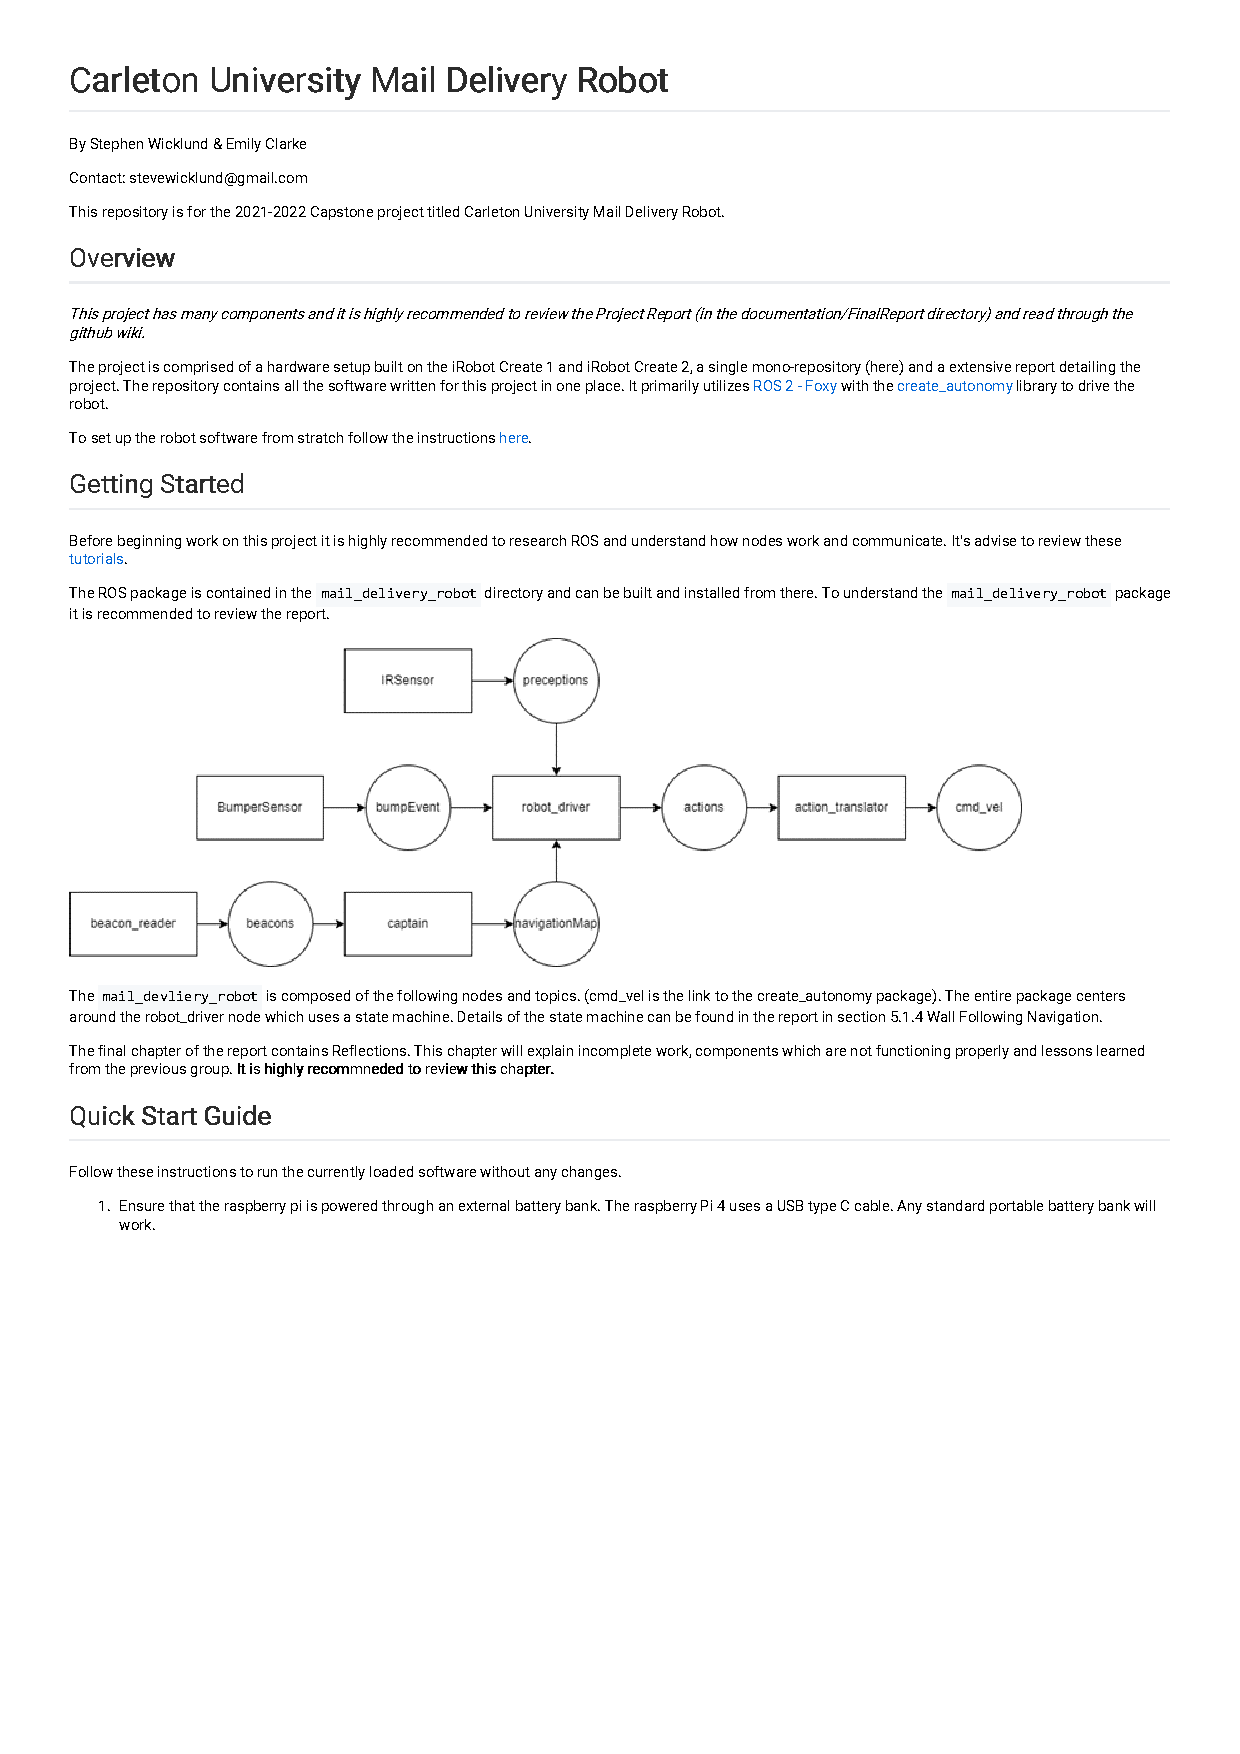
\includepdf[pages=-, offset=25 -75]{README.pdf}
\chapter{ROS 2 Setup}
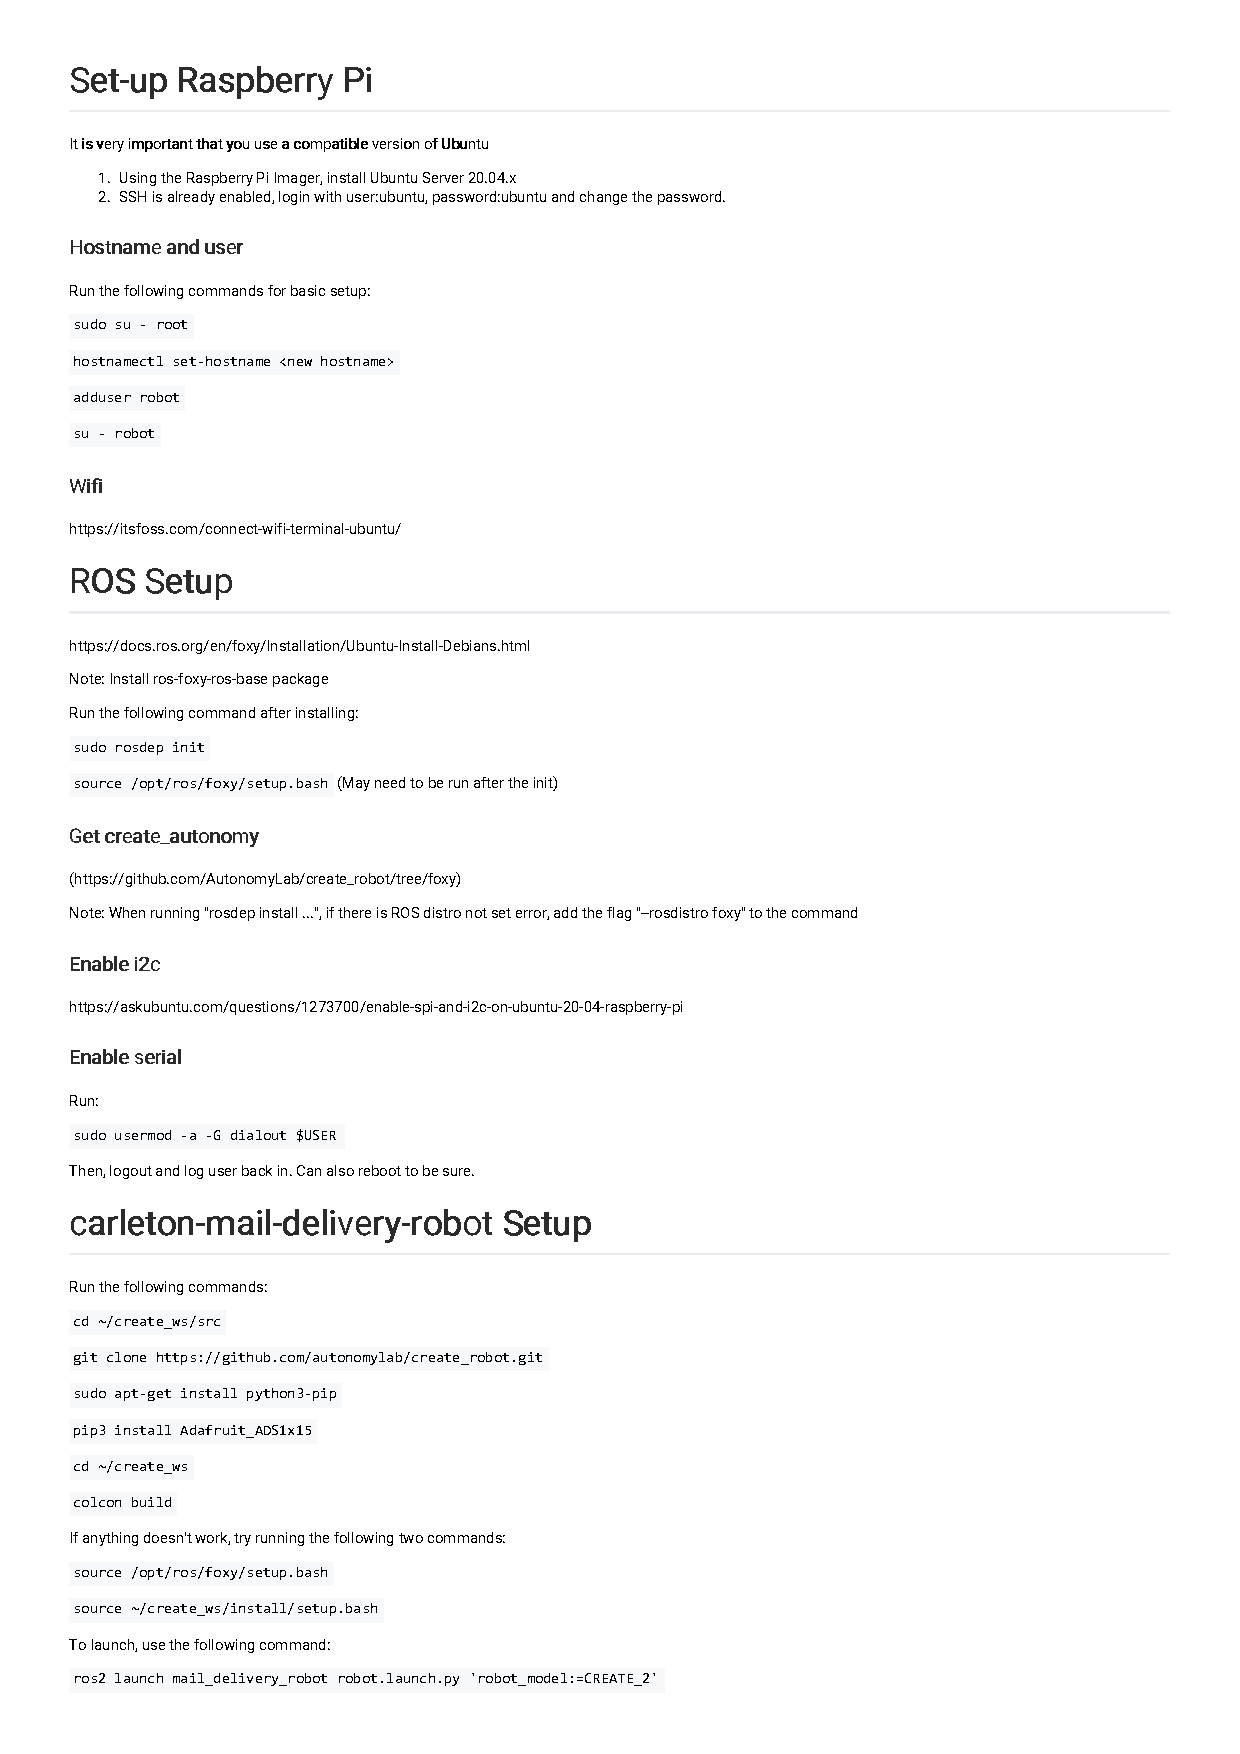
\includepdf[pages=-, offset=25 -75]{ROS2Setup.pdf}
\chapter{Beacon Setup}
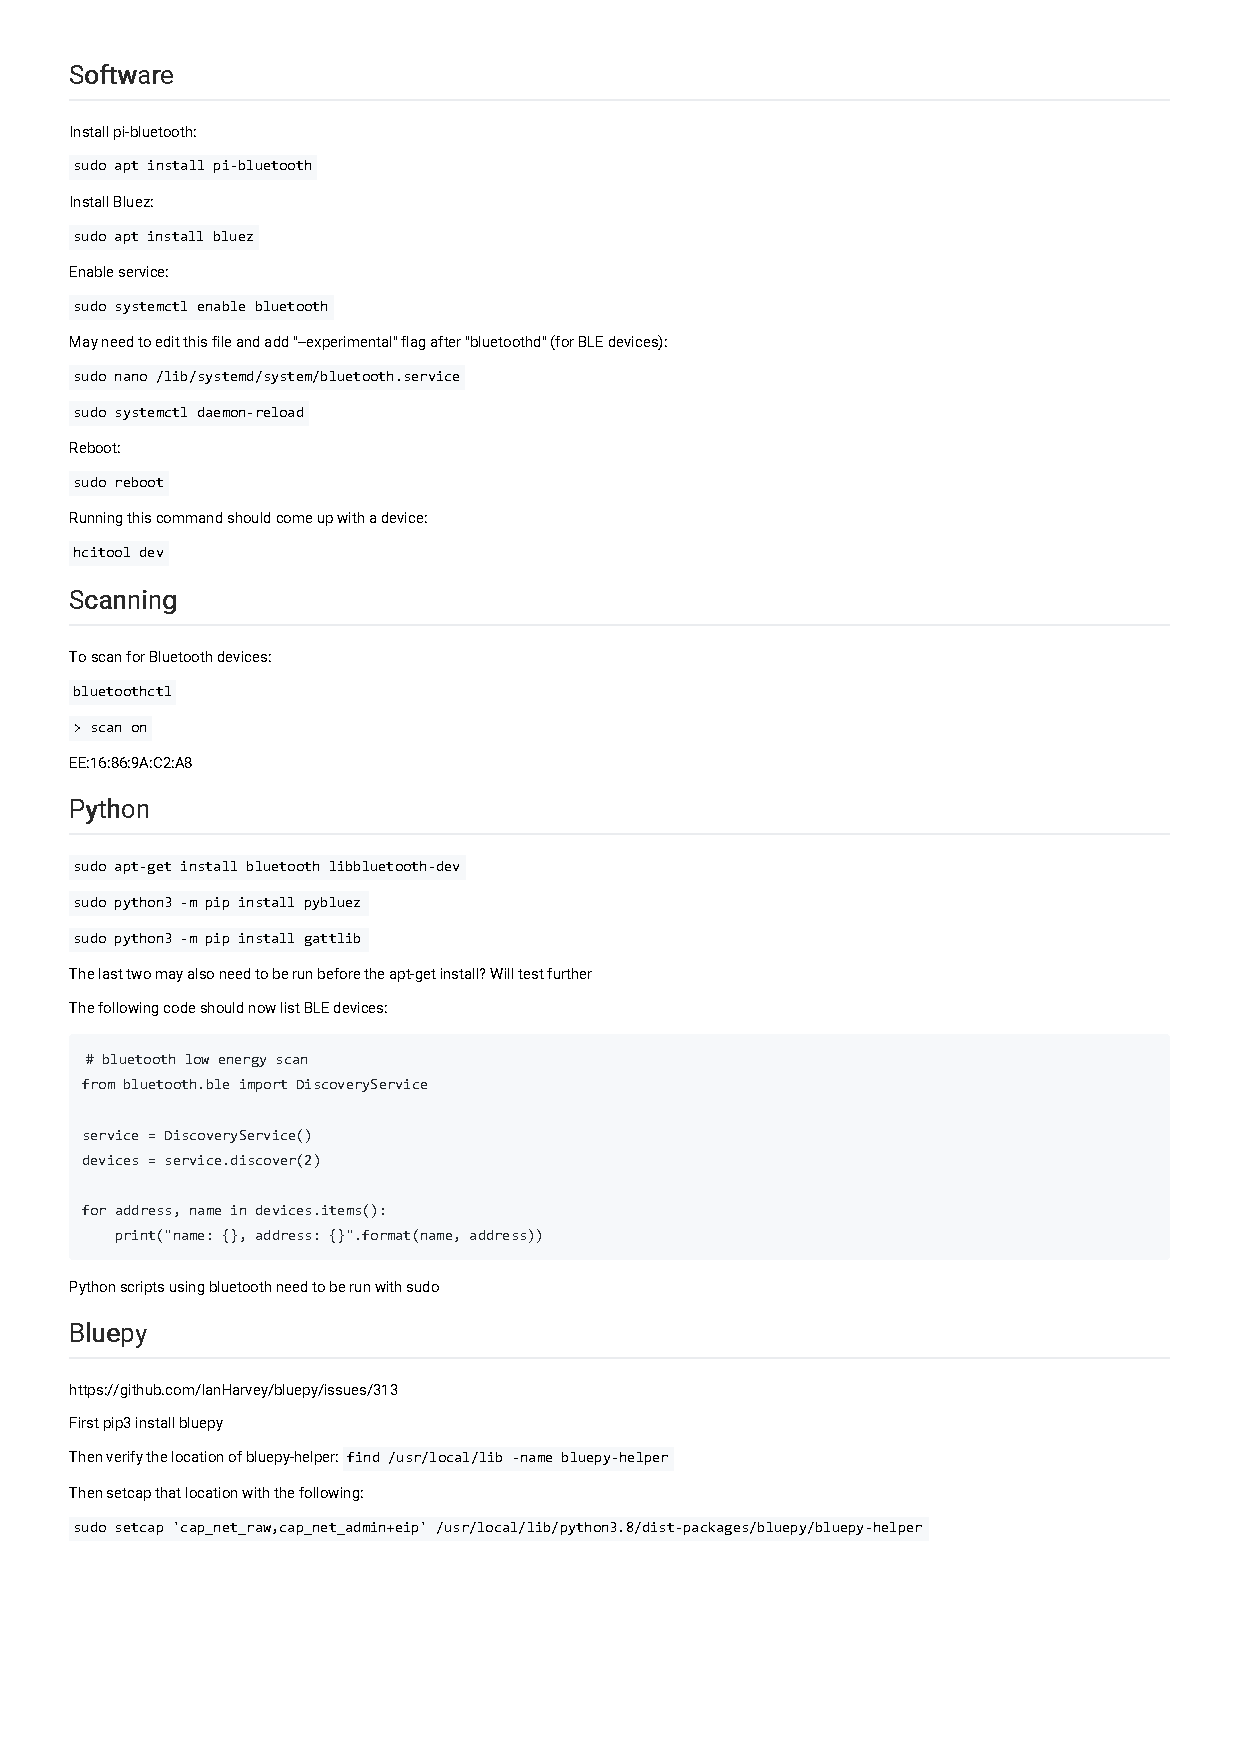
\includepdf[pages=-, offset=25 -75]{BeaconSetup.pdf}
\chapter{Fauna Database Setup}
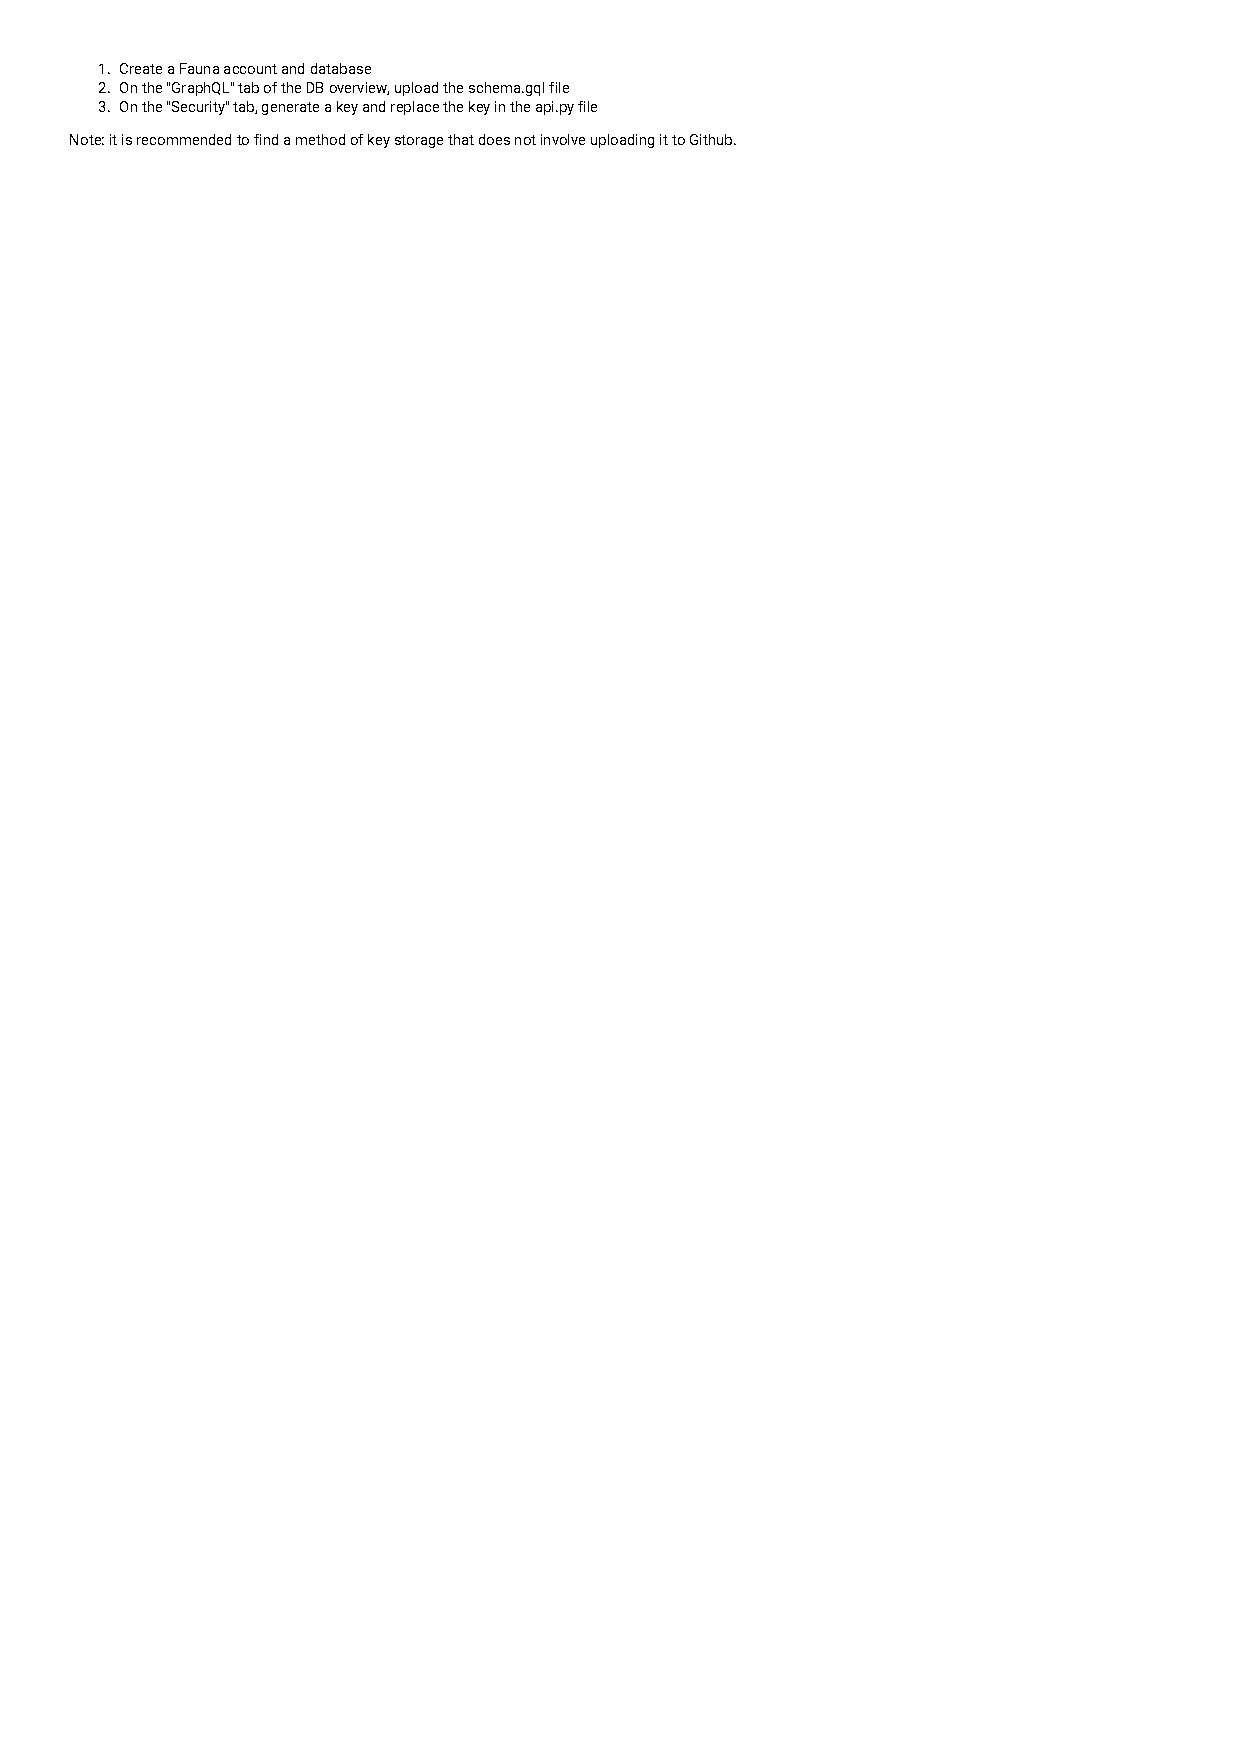
\includepdf[pages=-, offset=25 -75]{FaunaDatabaseSetup.pdf}
\end{document}
